\documentclass{report}
\usepackage{multicol}
\usepackage[T1]{fontenc}
\usepackage[utf8]{inputenc}
\usepackage{lmodern}
\usepackage{tikz}
\usepackage[a4paper,margin=2.5cm]{geometry}
\usepackage{amsmath,amssymb,amsthm}
\usepackage{graphicx}
\usepackage{booktabs}
\usepackage{siunitx}
\usepackage{enumitem}
\usepackage[table]{xcolor}
\usepackage[hidelinks]{hyperref}
\usepackage{float}
\usepackage[provide=*,italian]{babel}
\usepackage{biblatex}
\usepackage{csvsimple}
\addbibresource{DriftArchiDati.bib}
\newtheorem{definition}{Definizione}
\theoremstyle{definition}
\title{Report progetto Architetture Dati: data drift su ImageNet}
\author{Daniele Besozzi 894998, Andrea Consonni 900116, Elena Zen 895355}
\date{}
\begin{document}
\maketitle
\tableofcontents
\chapter{Introduzione al problema}
I sistemi di Machine Learning vengono generalmente sviluppati assumendo che i dati osservati durante l'addestramento siano rappresentativi di quelli che il modello incontrerà durante il suo utilizzo. Nelle applicazioni reali, tuttavia, questa assunzione è spesso disattesa: le caratteristiche della distribuzione dei dati possono variare nel tempo o tra differenti contesti di utilizzo. Questo fenomeno, comunemente indicato come \textbf{data drift} o \textbf{distribution shift}, può determinare una significativa riduzione delle prestazioni del modello anche in assenza di modifiche alla sua architettura o ai suoi parametri.

Lo studio della robustezza rispetto al \textbf{data drift} rappresenta pertanto un aspetto fondamentale nella valutazione di sistemi di Machine Learning. È infatti importante non limitarsi a misurare le prestazioni su dati provenienti dalla stessa distribuzione utilizzata in fase di training (\textbf{in-distribution}), ma valutare anche il comportamento del modello in presenza di variazioni nella distribuzione degli input (\textbf{out-of-distribution}). Tali variazioni possono assumere forme differenti, includendo cambiamenti nelle condizioni di acquisizione delle immagini, nella loro qualità, nello stile visivo o nella presenza di specifiche perturbazioni.

In questo progetto, l'effetto del \textbf{data drift} sulle prestazioni dei modelli di classificazione d'immagini è stato analizzato attraverso una serie di benchmark basati sulla famiglia di dataset ImageNet. In particolare, sono stati considerati \textbf{ImageNet}, utilizzato come riferimento per la valutazione \textbf{in-distribution}, \textbf{ImageNet-R}, progettato per valutare la robustezza del modello rispetto a variazioni nella rappresentazione visiva degli oggetti, e \textbf{ImageNet-C}, che introduce diverse tipologie di corruzioni comuni applicate alle immagini. La combinazione di questi benchmark consente di analizzare il comportamento del modello in presenza di forme differenti di \textbf{distribution shift}, distinguendo tra variazioni di stile e rappresentazione e perturbazioni che simulano degradazioni o condizioni avverse nell'acquisizione dei dati.

L'obiettivo dell'analisi è quindi quantificare quanto il cambiamento nella distribuzione degli input influenzi le prestazioni del modello rispetto allo scenario di riferimento.
\section{Definizioni di data drift}
Nel machine learning supervisionato applicato a scenari reali, l'assunzione fondamentale per garantire la capacità di generalizzazione di un modello è che i dati di addestramento e i dati su cui il modello opererà una volta rilasciato siano indipendenti e identicamente distribuiti (i.i.d.)\cite{moreno-torres_unifying_2012, tamang_handling_2025}. Tuttavia, negli scenari applicativi reali, questa assunzione teorica viene costantemente violata. Le discrepanze tra l'ambiente controllato di laboratorio e le condizioni dinamiche del mondo reale, indotte da fattori quali distorsioni nella raccolta dei dati (sample selection bias), ambienti non stazionari o evoluzioni temporali e spaziali, causano variazioni nelle distribuzioni dei dati.

La letteratura scientifica ha storicamente sofferto di una frammentazione terminologica, utilizzando in modo intercambiabile nomi diversi per definire concetti analoghi (es. concept drift, population drift, changing environments, data fracture)\cite{moreno-torres_unifying_2012}. In questo progetto adottiamo la seguente definizioni proposte da Moreno-Torres et al. \cite{moreno-torres_unifying_2012}:
\begin{definition}[Dataset shift]
	Si verifica quando la distribuzione di probabilità congiunta delle feature (o covariate) $x$ e della variabile target (classe) $y$ differisce tra la fase di addestramento ($P_{tr}$) e la fase di test ($P_{tst}$).
	Formalmente, $P_{tr}(y,x) \neq P_{tst}(y,x)$.
\end{definition}
Per poter analizzare e risolvere questo problema, è necessario distinguere la direzione causale tra la classe $y$ e le feature $x$. Si identificano quindi due classi di problemi:
\begin{itemize}
	\item Problemi $X\rightarrow Y$, in cui la classe $y$ è determinata causalmente dal valore delle feature $x$ (es. la rilevazione delle frodi bancarie, dove il comportamento dell'utente determina se c'è una frode).
	\item Problemi $Y\rightarrow X$, in cui la classe $y$ determina causalmente il valore delle feature $x$ (tipico della diagnostica medica, in cui la patologia $y$ causa i sintomi osservabili $x$)
\end{itemize}\
\section{Tipologie di data drift}
Il data drift può manifestarsi in diverse forme, a seconda della natura delle variazioni nella distribuzione dei dati. In questa sezione presentiamo le principali tipologie di data drift identificate in letteratura.
\subsection{Covariate shift (o Population Drift)}
Il covariate shift si riferisce al cambiamento della distribuzione delle variabili di input (o covariate) $x$ tra la fase di training e quella di test, mentre la relazione condizionata che mappa l'input alla classe rimane del tutto invariata.
Formalmente:
\begin{definition}[Covariate shift]
	Appare solamente nei problemi del tipo $X \rightarrow Y$ e si verifica nel caso in cui
$P_{tr}(x) \neq P_{tst}(x)$ e $P_{tr}(y|x) = P_{tst}(y|x)$
\end{definition}
Ad esempio, un modello di classificazione d'immagini addestrato principalmente su foto di cani su uno sfondo erboso che viene poi testato su immagini di cani che indossano impermeabili in contesti urbani \cite{tamang_handling_2025}. Le feature visive di sfondo e i dettagli superficiali cambiano ($P(x)$ muta), ma il concetto semantico di "cane" associato a quelle immagini rimane lo stesso ($P(y|x)$ è costante).	
\begin{figure}[H]
	\centering
	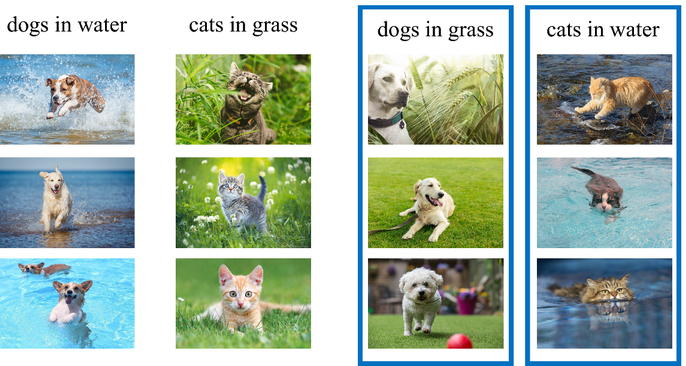
\includegraphics[width=0.8\textwidth]{images/covariate_shift.png}
	\caption{Esempio di covariate shift}
	\label{fig:covariate_shift}
\end{figure}
\subsection{Prior probability shift}
Il prior probability shift rappresenta il caso duale del covariate shift, focalizzato sul cambiamento della distribuzione della variabile target $y$, mentre la distribuzione condizionata delle feature data la classe rimane costante.
Formalmente:
\begin{definition}[Prior probability shift]
	Appare solamente nei problemi del tipo $Y \rightarrow X$ e si verifica nel caso in cui $P_{tr}(y) \neq P_{tst}(y) $ e $P_{tr}(x|y) = P_{tst}(x|y)$.
\end{definition}
Ad esempio, in un sistema di diagnostica medica per una specifica malattia infettiva, la distribuzione dei sintomi per i soggetti malati e sani rimane costante ($P(x|y)$ non cambia), ma la prevalenza complessiva della malattia nella popolazione $P(y)$ fluttua nel tempo (ad esempio, a causa di un'improvvisa epidemia o di una campagna vaccinale).
\subsection{Concept Shift (o Concept Drift)}
Il concept shift (o concept drift) si verifica quando cambia la relazione funzionale o semantica tra le feature di input e la variabile target, modificando di fatto la definizione stessa della classe da apprendere. Rappresenta la sfida più complessa, poiché i criteri decisionali appresi dal modello durante l'addestramento non sono più validi nell'ambiente operativo.
Formalmente:
\begin{definition}[Concept shift] Si verifica nel caso in cui:
	$$
		\begin{aligned} P_{tr}(y|x) \neq P_{tst}(y|x) \quad \text{e} \quad P_{tr}(x) = P_{tst}(x) & \quad (\text{nei problemi }X\rightarrow Y) \\ P_{tr}(x|y) \neq P_{tst}(x|y) \quad \text{e} \quad P_{tr}(y) = P_{tst}(y) & \quad (\text{nei problemi } Y \rightarrow X) \end{aligned}
	$$
\end{definition}
Ad esempio, nei sistemi di filtraggio dello spam o di rilevamento delle intrusioni di rete, gli utenti malintenzionati modificano attivamente le proprie strategie per eludere i filtri esistenti, cambiando la definizione di ciò che costituisce un'e-mail di spam o un attacco, lasciando però apparentemente inalterata la struttura generale del traffico dati.
\section{Cause del drift}
Si possono rilevare due principali cause del data drift:
\begin{itemize}
	\item \textbf{Sample Selection Bias}:
	Avviene quando il metodo di campionamento o di etichettatura dei dati di addestramento non è uniforme o casuale rispetto alla popolazione reale.
	\item \textbf{Ambienti Non Stazionari }: Molti contesti operativi sono intrinsecamente dinamici nel tempo e nello spazio. 
	In generale, gli ambienti sono dinamici e, talvolta, la difficoltà nel far corrispondere lo scenario di apprendimento all'utilizzo nel mondo reale è dovuta proprio a questi cambiamenti. Tali scenari rendono complesso valutare l'adeguatezza di uno specifico modello in presenza di variazioni ambientali, aumentando così la probabilità di shift.
	
\end{itemize}
\chapter{Analisi dei dataset}
Per valutare e quantificare la capacità di generalizzazione Out-of-Distribution (OOD) del modello analizzato in questo progetto, abbiamo strutturato i test utilizzando tre dataset della famiglia ImageNet. In particolare, abbiamo utilizzato i dataset ImageNet-1k, ImageNet-C e ImageNet-R.
In questo capitolo, descriveremo le caratteristiche principali di ciascun dataset e le motivazioni che ci hanno portato a sceglierli per i nostri test.
\section{ImageNet}
ImageNet è un ampio dataset d'immagini etichettate, ampiamente utilizzato per addestrare e valutare modelli di visione artificiale. Contiene oltre 14 milioni d'immagini annotate con più di 20.000 categorie di oggetti.
La costruzione del dataset è stata effettuata in tre fasi:
\begin{enumerate}
	\item \textbf{Mappatura WordNet}: per strutturare il dataset è stata usata la struttura gerarchica di WordNet, un database lessicale che organizza le parole in insiemi di sinonimi (synsets) e le collega tra loro attraverso relazioni semantiche. Ogni synset ha un "WordNet ID" (WNID) univoco, che è stato utilizzato per etichettare le immagini nel dataset. In questo modo, le immagini sono state organizzate in categorie gerarchiche basate sui synset di WordNet.
	\item \textbf{Web scraping}: le immagini sono state raccolte da Internet utilizzando tecniche di web scraping. Sono stati utilizzati motori di ricerca e altre fonti online per raccogliere immagini pertinenti alle categorie di oggetti definite dai synset di WordNet.
	\item \textbf{Annotazione manuale}: le immagini raccolte sono state annotate manualmente attraverso il servizio Amazon Mechanical Turk(AMTurk). Ogni immagine è stata etichettata con la categoria di oggetti corretta, garantendo così l'accuratezza delle annotazioni.
\end{enumerate}
Il database completo originario è noto come ImageNet-21K (o ImageNet-22K) e contiene circa 14,2 milioni d'immagini distribuite su 21.841 classi gerarchiche. Non è presente uno split training-validation-test ufficiale. Il dataset non è bilanciato: alcune classi contengono un numero molto basso di esempi, mentre altre classi contengono un numero elevato di esempi.
\section{ImageNet-1k}
Vengono spesso utilizzati subset di ImageNet-21k per vari scopi. 
Uno dei più noti è ImageNet-1k, che contiene 1.000 classi di oggetti selezionate da ImageNet-21k. Il dataset contiene 1.281.167 immagini di training, 50.000 immagini (50 per classe) di validation e 100.000 immagini di test.

Questo dataset è stato utilizzato per addestrare e valutare modelli di visione artificiale, in particolare per la competizione ImageNet Large Scale Visual Recognition Challenge (ILSVRC). Per questo motivo, il test set non è etichettato, in quanto serve unicamente a valutare le prestazioni dei modelli durante la competizione. Perciò, per i nostri test, abbiamo utilizzato il validation set come test set, questo è possibile in quanto il validation set non viene utilizzato per l'addestramento del modello, ma solo per la valutazione delle sue prestazioni\cite{he_deep_2016}.

A differenza della struttura gerarchica ad albero di ImageNet-21K (che include macro-classi come "mammifero" o "veicolo"), ImageNet-1K contiene esclusivamente 1.000 classi non sovrapposte poste alla base dell'albero gerarchico (es. singole razze di cani come "German shepherd", senza includere la classe genitore "dog")
\section{ImageNet-C}
A differenza di altri dataset, ImageNet-C non è stato raccolto fotografando nuovi oggetti o facendo web scraping. È stato costruito applicando sistematicamente corruzioni digitali e matematiche direttamente sul set di validazione originale di ImageNet-1K (le 50.000 immagini di validazione)
L'obiettivo dei creatori era imitare le reali limitazioni fisiche dei sensori delle fotocamere, le variazioni atmosferiche ambientali e i disturbi dovuti alla compressione e trasmissione dei dati, escludendo però alterazioni avversariali mirate (worst-case)\cite{hendrycks_benchmarking_2019}.
Il dataset si sviluppa in modo gerarchico:
\begin{itemize}
	\item \textbf{Corruzioni}: sono state applicate 15 corruzioni digitali e matematiche, suddivise in 4 categorie principali: \textit{blur}, \textit{noise}, \textit{digital} e \textit{weather}. 
	\begin{itemize}
		\item \textit{Blur}: motion blur, defocus blur, frosted glass blur, gaussian blur, zoom blur
		\item \textit{Noise}: gaussian noise, shot noise, impulse noise
		\item \textit{Digital}: brightness, contrast, elastic transform, pixelate, jpeg compression
		\item \textit{Weather}: snow, frost, fog
	\end{itemize}
	\item \textbf{Intensità}: per ogni corruzione sono stati generati 5 livelli di intensità, da 1 (minima) a 5 (massima).
\end{itemize}
La dimensione totale del test set di ImageNet-C è quindi di $50.000 \times 15 \text{ corruzioni} \times 5 \text{ severità} = 3.750.000$ immagini di test.
\begin{figure}[H]
	\centering
	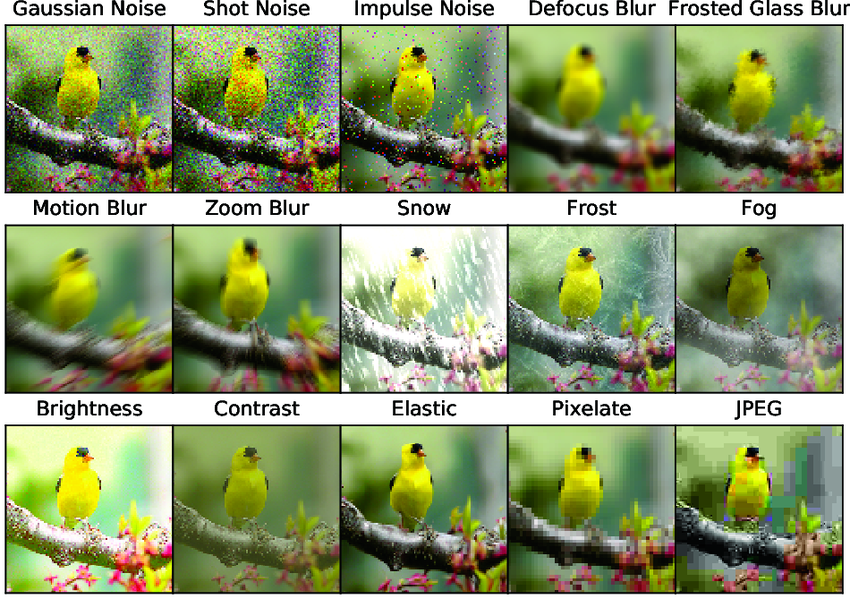
\includegraphics[width=0.8\textwidth]{images/ImageNetC_example.png}
	\caption{Esempi di corruzioni applicate a un'immagine del dataset ImageNet-1K.}
	\label{fig:imagenet_c}
\end{figure}
\section{ImageNet-R}
ImageNet-R è un dataset di immagini raccolte da Internet, progettato per testare la capacità di generalizzazione dei modelli di visione artificiale su immagini stilizzate e artistiche. Il dataset è stato creato seguendo le seguenti procedure descritte in \cite{hendrycks_many_2021}:
\begin{enumerate}
	\item \textbf{Sottocampionamento delle classi}: Gli autori hanno selezionato un subset di 200 classi di ImageNet-1K. Ciò è stato necessario a causa della difficoltà di trovare immagini stilizzate per tutte le 1.000 classi di ImageNet-1K, dunque sono state selezionate solo le classi per le quali era possibile reperire un numero sufficiente d'immagini stilizzate. Inoltre sono state scelte classi facilmente riconoscibili da un umano, ad esempio "cane" invece che indicare una razza specifica di cane.
	\item \textbf{Raccolta delle immagini}: Le immagini sono state ottenute tramite scraping da Flickr, fonte da cui erano state ottenute parte delle immagini di ImageNet-1K. 
	\item \textbf{Filtro di Qualità Manuale}:

    \begin{itemize}
		\item I lavoratori di Amazon Mechanical Turk hanno eseguito una prima scrematura scartando i falsi positivi (immagini non coerenti con la classe semantica cercata).
		\item Un team di studenti di dottorato ha eseguito una revisione manuale finale, eliminando le immagini con etichette ambigue o multiple per garantire che ogni immagine avesse un'unica classe definita e corretta
	\end{itemize} 
\end{enumerate}
Il dataset finale contiene 30.000 immagini di test, con un numero variabile d' immagini per classe, da un minimo di 51 a un massimo di 430 immagini per classe, in media 150 immagini per classe.
Le immagini sono categorizzate in base a diversi stili (es. Painting, Sculpture, Origami, Cartoon, Toy, Embroidery, ecc.). Ai fini della classificazione, le etichette di destinazione rimangono quelle semantiche di ImageNet-1K.
\begin{figure}[H]
	\centering
	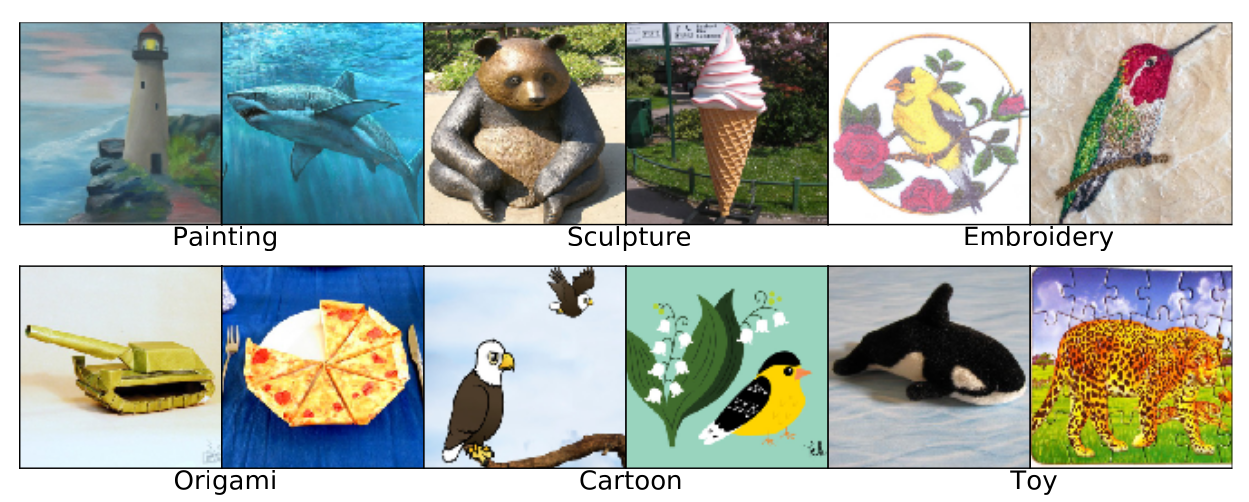
\includegraphics[width=0.8\textwidth]{images/ImageNetR_example.png}
	\caption{Esempi di immagini stilizzate del dataset ImageNet-R. Painting, etc. sono stili di rappresentazione, non etichette.}
	\label{fig:imagenet_r}
\end{figure}
\chapter{Introduzione al modello}

Ogni tipo di modello di machine learning supervisionato può riscontrare, quando si trova ad operare
in contesti reali, un drift nelle distribuzioni dei dati osservati rispetto alla distribuzione
osservata durante la fase di addestramento. In particolare, uno dei tipi di modello più diffuso per il riconoscimento
delle immagini è quello che prende il nome di \textbf{rete neurale convolutiva} (Convolutional neural network, CNN).
In questo capitolo, introdurremo il funzionamento delle CNN e descriveremo l'architettura
utilizzata per questo progetto, le \textbf{reti neurali residuali}.
\section{Reti neurali convolutive}
Le \textbf{reti neurali convolutive} furono per la prima volta introdotte nella loro
forma moderna nel 1989 da Le Cun et al \cite{lecun_handwritten_1989}, i quali svilupparono LeNet-5, una
rete convolutiva in grado di classificare le cifre scritte a mano su dei fogli.
La struttura particolare di questo tipo di reti le rende particolarmente efficaci nell'ambito
del riconoscimento di immagini, poiché esse sono capaci di sfruttare le \textbf{caratteristiche spaziali dell'input}, come
per esempio la correlazione spaziale tra pixel vicini. Questa caratteristica permette inoltre di \textbf{ridurre il numero di pesi necessari da imparare},
rendendo quindi la rete più efficiente.
La figura \ref{fig:cnn_example} mostra l'architettura di LeNet-5 come esempio di rete neurale convolutiva.
Oltre ai layer di input e di output, le reti neurali convolutive sono formate principalmente da tre tipi di strati \cite{oshea_introduction_2015}:
\begin{itemize}
    \item Strati convolutivi
    \item Strati di pooling (o di subsampling)
    \item Strati completamente connessi
\end{itemize}
\begin{figure}
    \centering
    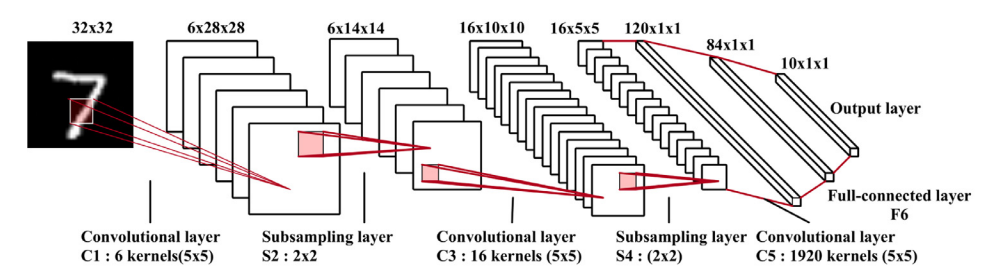
\includegraphics[width = \textwidth]{images/le-net.png}
    \caption{Architettura di LeNet-5. Da \cite{gu_recent_2018}}
    \label{fig:cnn_example}
\end{figure}
\subsubsection{Strato di input}
Come nelle reti neurali tradizionali, lo strato di input di una rete neurale convolutiva conterrà i valori delle istanze
che verranno passate alla rete. In particolare per le immagini, essi sono i \textbf{valori numerici dei suoi pixel}. Possiamo
quindi vedere un'immagine come una matrice di dimensioni $W \times H \times C$, con $W$ la larghezza dell'immagine, $H$ l'altezza dell'immagine
e $C$ il numero di \textbf{canali colore} (per esempio, $C =3$ se l'immagine ha canali colore RGB).
\subsubsection{Strati convolutivi}
Come abbiamo già detto sopra, le reti neurali convolutive sono in grado di sfruttare la struttura spaziale dell'input. Questo avviene nei \textbf{layer convolutivi}, il cui scopo è quello di imparare delle \textbf{rappresentazioni delle feature dell'input} \cite{gu_recent_2018}, cioè una rappresentazione delle caratteristiche presenti all'interno dell'input. Nel contesto delle immagini, esse possono essere, ad esempio, bordi, angoli, texture e forme.
L'apprendimento e l'estrazione di tali caratteristiche vengono effettuati avvalendosi di diversi \textbf{kernel convolutivi} (o filtri convolutivi), i quali vengono appresi dalla rete e utilizzati per effettuare una \textbf{convoluzione} sull'immagine. Più precisamente, il kernel viene fatto scorrere sull'input, considerando a ogni posizione una piccola regione locale di esso. Tale regione, rispetto al neurone che ne riceve le informazioni, viene definita \textbf{receptive field}. Viene quindi effettuato il prodotto scalare tra i valori presenti in questa regione e i pesi del kernel, ottenendo il valore di ingresso del neurone, il quale applicherà ad esso una funzione di attivazione non lineare per ottenere il suo valore di output, cioè la sua \textbf{attivazione}. Ripetendo questa operazione nelle diverse posizioni spaziali dell'input si ottiene una \textbf{feature map}, nella quale ogni valore corrisponde all'attivazione di un neurone in corrispondenza di una specifica regione dell'input. Ogni layer convolutivo si avvale di più kernel, i quali produrranno una feature map diversa ciascuno. Questo meccanismo ha diversi vantaggi:
\begin{itemize}
    \item Lo stesso kernel viene \textbf{condiviso tra tutte le posizioni spaziali dell'input}: in questo modo, lo stesso insieme di pesi viene utilizzato per rilevare una determinata caratteristica indipendentemente dalla sua posizione nell'immagine. Ciò inoltre diminuisce la complessità del modello, facilitandone l'addestramento.
    \item L'utilizzo di kernel differenti permette di ottenere diverse feature map, ciascuna delle quali può rappresentare una diversa caratteristica appresa dall'input
\end{itemize}
La figura \ref{fig:feature_maps} mostra un esempio di estrazione di feature maps in una CNN.
\begin{figure}
    \centering
    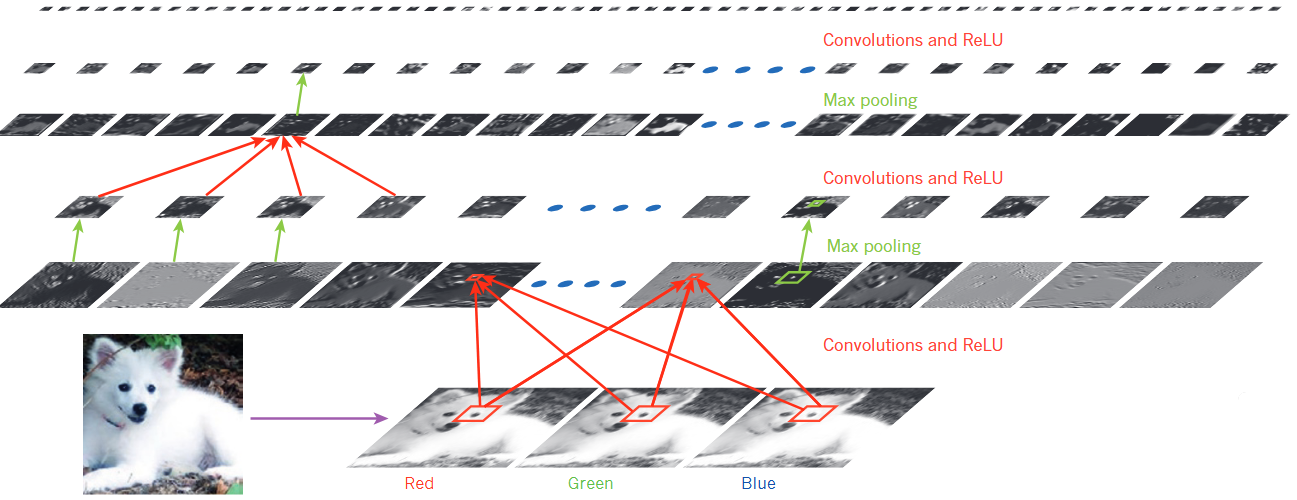
\includegraphics[width = \textwidth]{images/feature maps.png}
    \caption{Esempio di estrazione di feature map da un'immagine. Da \cite{lecun_deep_2015}}
    \label{fig:feature_maps}
\end{figure}
Infine, il kernel viene spostato sull'immagine di una quantità chiamata \textbf{stride}, che rappresenta il numero di pixel di cui il kernel viene traslato a ogni operazione di convoluzione. Di conseguenza, aumentando lo stride diminuisce il numero di posizioni nelle quali il kernel viene applicato e, in generale, si ottiene una \textbf{feature map} di dimensioni spaziali inferiori. Se i kernel della rete sono troppo grandi rispetto alle dimensioni dell'input, si può inoltre introdurre dello \textbf{zero padding} ai suoi bordi.
\subsubsection{Strati di pooling}
Lo scopo degli strati di pooling è quello di \textbf{ridurre le dimensioni spaziali delle feature map ottenute dai layer convolutivi} e, di conseguenza, ridurre la complessità computazionale del modello \cite{oshea_introduction_2015}. Anche questi layer si avvalgono di kernel per operare su piccole regioni spaziali dell'input. Tuttavia, a differenza degli strati convolutivi, questi kernel non possiedono parametri apprendibili e applicano generalmente una delle seguenti operazioni:
\begin{itemize}
    \item \textbf{Max-pooling}: viene selezionato il valore massimo tra quelli contenuti nella regione considerata.
    \item \textbf{Average-pooling}: viene calcolata la media dei valori contenuti nella regione considerata.
\end{itemize}
L'output di un layer di pooling sarà quindi una nuova \textbf{feature map} con dimensioni spaziali ridotte rispetto a quella in ingresso.  I layer di pooling sono generalmente posti tra due layer convolutivi e operano indipendentemente su ciascuna feature map. Combinando diversi layer convolutivi e di pooling, la rete può progressivamente estrarre caratteristiche sempre più complesse e di alto livello \cite{gu_recent_2018}.
\subsubsection{Strati completamente connessi}
% TODO: ricontrollare
Come in una rete neurale tradizionale, gli strati completamente connessi si occupano di \textbf{combinare le informazioni provenienti dallo strato precedente}, collegando ciascun neurone a tutti i neuroni dello strato precedente. In questo modo, le caratteristiche estratte dai layer convolutivi e vengono integrate per ottenere una rappresentazione globale dell'input \cite{gu_recent_2018}, che può essere successivamente utilizzata per effettuare la classificazione.
\subsubsection{Strato di ouput}
L'ultimo strato di una rete neurale convolutiva è lo strato di output, il quale si occupa di restituire il risultato della classificazione. Spesso, questo strato è rappresentato dall'operatore \textbf{softmax} oppure da una \textbf{SVM} \cite{gu_recent_2018}.
\section{Reti neurali residuali}
Le \textbf{reti neurali residuali} sono un'architettura per reti neurali profonde, proposto per la prima volta nel 2016 da He et al. \cite{he_deep_2016} e progettata per affrontare il problema della \textbf{degradazione}. Tale fenomeno si manifesta quando l'aumento della profondità della rete, ovvero del numero di layer, porta inizialmente a una saturazione dell'accuratezza e successivamente a un suo rapido decremento. Questo problema, inoltre, non è causato dall'overfitting, quindi aggiungere più layer alla rete porta ad un errore maggiore durante l'addestramento.  Per combattere questo fenomeno, le reti residuali adottano le seguenti soluzioni:
\begin{itemize}
    \item \textbf{Apprendimento residuale}: Consideriamo un insieme di layer di una rete neurale e supponiamo di voler fare in modo che essi apprendano un determinato mapping $\mathcal{H}(\boldsymbol{x})$, dove $\boldsymbol{x}$ rappresenta l'input fornito al primo dei layer considerati. Anziché apprendere direttamente il mapping desiderato, facciamo apprendere ai layer il \textbf{mapping residuale} $\mathcal{F}(\boldsymbol{x})$, definito come:
    $$\mathcal{F}(\boldsymbol{x}) \coloneqq \mathcal{H}(\boldsymbol{x}) - \boldsymbol{x}$$
    Di conseguenza, il mapping originale diventa:
    $$\mathcal{H}(\boldsymbol{x}) = \mathcal{F}(\boldsymbol{x}) + \boldsymbol{x}$$
    Questa riformulazione è giustificata dalla natura controintuitiva del problema della degradazione: la manifestazione di questo problema potrebbe indicare che i solver di ottimizzazione faticano ad approssimare l'identità componendo più layer non lineari. Riformulando il mapping in questo modo, l'ottimizzazione diventa più semplice: se il mapping ottimale è vicino all'identità, è sufficiente che i pesi dei layer tendano a zero.
    \item \textbf{Identity shortcut connections}: Il mapping $\mathcal{F}(\boldsymbol{x}) + \boldsymbol{x}$ può essere realizzato da una rete dotata di "shortcut connections", ovvero connessioni che saltano uno o più layer della rete. Nel caso delle reti residuali, queste connessioni collegano semplicemente l'input di un gruppo di layer alla sua uscita, sommando l'identità $\boldsymbol{x}$ all'output dei layer.
\end{itemize}
\begin{figure}
    \centering
    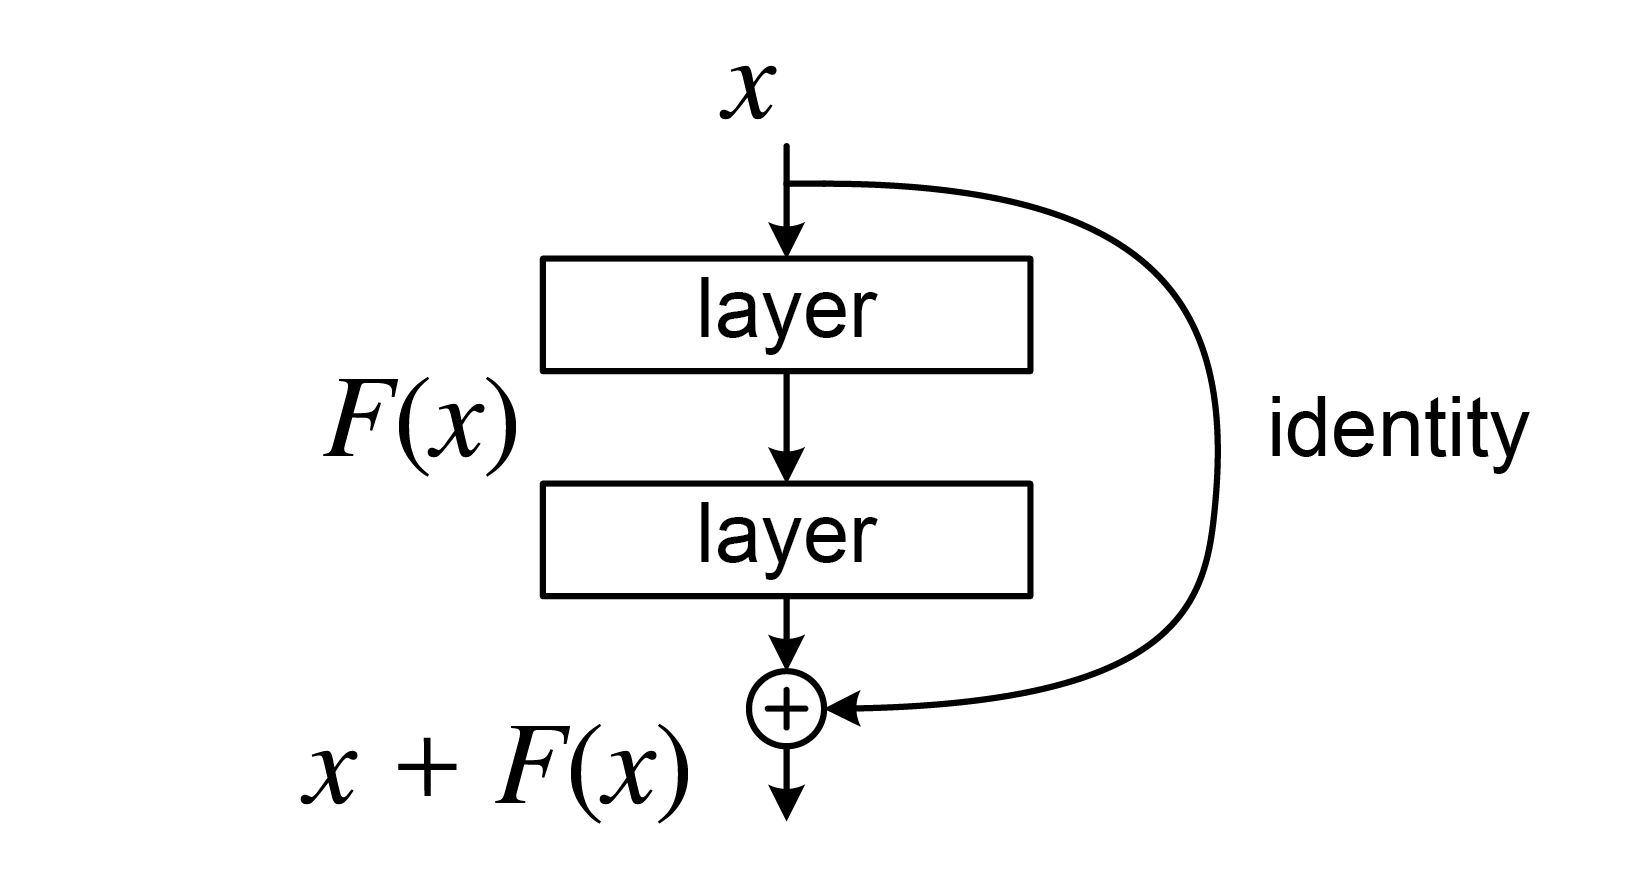
\includegraphics[width = 0.55\textwidth]{images/resnet.png}
    \caption{Esempio di blocco residuale. Da \cite{he_deep_2016}}
    \label{fig:residual_block}
\end{figure}
La figura \ref{fig:residual_block} mostra un esempio di blocco residuale. Queste soluzioni portano ad ottenere reti più facili da ottimizzare rispetto alle reti neurali profonde tradizionali e in grado di trarre maggiore beneficio, in termini di accuratezza, dall'aumento della profondità.
\subsection{ResNet50}
I modelli sviluppati da He et al. in \cite{he_deep_2016} sono stati addestrati e valutati su ImageNet-1k. Uno di questi modelli è ResNet50, il quale viene utilizzato come modello per questo progetto.  
Le versioni di rete residuale più profonde, tra cui ResNet50, adottano un blocco residuo differente rispetto a quello base a due layer utilizzato nelle versioni meno profonde: per contenere i tempi di addestramento, ogni funzione residuale $\mathcal{F}$ viene realizzata tramite tre layer convolutivi di dimensioni rispettivamente $1 \times 1$, $3 \times 3$ e $1 \times 1$, detti \textbf{layer di bottleneck}. Il primo e l'ultimo layer si occupano rispettivamente di ridurre e successivamente ricostruire le dimensioni dell'input, mentre il layer $3 \times 3$ centrale opera come un "collo di bottiglia" (\textit{bottleneck}), con dimensioni di input e output ridotte rispetto al resto del blocco. Questo cambiamento non comporta nessun aumento significativo della complessità computazionale, la quale resta simile rispetto all'implementazione a due blocchi. Un esempio di blocco "bottleneck" è mostrato in figura \ref{fig:bottleneck}
\begin{figure}
    \centering
    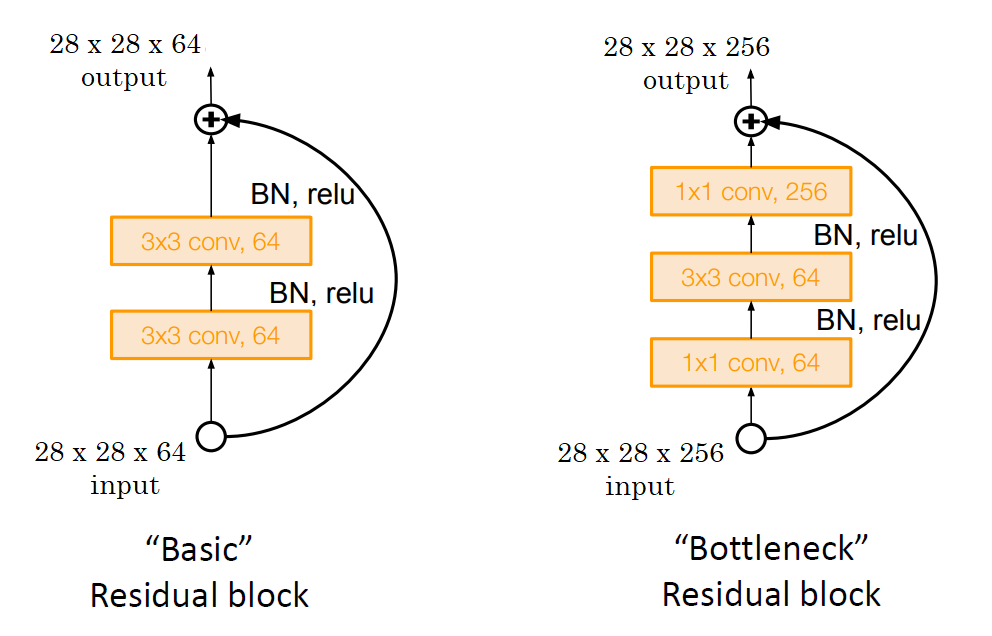
\includegraphics[width = 0.65\textwidth]{images/bottleneck.PNG}
    \caption{Confronto tra un blocco residuale e un blocco "bottleneck". Da \cite{he_deep_2016}}
    \label{fig:bottleneck}
\end{figure}
\chapter{Presentazione della metodologia}

In questa sezione descriviamo la metodologia adottata per valutare la capacità di generalizzazione Out-of-Distribution (OOD) del modello analizzato. Il processo si articola in tre fasi principali: preprocessing dei dataset, testing del modello e analisi del drift.

\section{Librerie e strumenti utilizzati}
Il progetto è stato sviluppato in Python 3.12 e fa uso delle seguenti librerie principali:

\begin{itemize}
	\item \textbf{PyTorch (torch) e TorchVision}: per il caricamento del modello ResNet-50 pre-addestrato, la definizione della pipeline di preprocessing e l'esecuzione dell'inferenza sulle GPU.
	\item \textbf{HuggingFace Datasets}: per il caricamento, la trasformazione e la gestione efficiente dei dataset ImageNet-1k, ImageNet-R e ImageNet-C in formato Arrow, con supporto al parallelismo e alla serializzazione su disco.
	\item \textbf{NumPy e Pandas}: per la manipolazione numerica e tabulare dei dati, inclusa la gestione delle feature estratte e dei risultati delle metriche.
	\item \textbf{Scikit-learn}: per il calcolo delle metriche di classificazione (accuracy, balanced accuracy, precision, recall, F1-score, MCC, Cohen's Kappa).
	\item \textbf{SciPy}: per la stima della densità kernel (\texttt{gaussian\_kde}), l'integrazione numerica (\texttt{trapezoid}), la regressione lineare (\texttt{linregress}) e la distribuzione $t$ di Student per gli intervalli di confidenza.
	\item \textbf{Evidently}: libreria open-source per il monitoraggio e la rilevazione del data drift. È stata utilizzata per eseguire i test di Wasserstein (normed) sulle proprietà visive delle immagini e il test \texttt{empirical\_mmd} sulle feature estratte dal modello.
	\item \textbf{Matplotlib e Seaborn}: per la visualizzazione dei risultati, inclusi grafici KDE di distribuzione delle proprietà delle immagini, andamenti delle metriche al vari della severità delle corruzioni e diagrammi a barre per il confronto baseline vs drift.
	\item \textbf{Pillow (PIL)}: per l'estrazione delle proprietà visive delle immagini (luminosità, contrasto RMS, nitidezza, rapporto d'aspetto, area, media dei canali RGB).
	\item \textbf{tqdm}: per le barre di progresso durante l'estrazione delle proprietà e l'esecuzione dell'inferenza.
\end{itemize}

\section{Preprocessing dei dataset}
Il preprocessing è gestito dallo script \texttt{data\_preprocess/datasets\_preprocess.py}, che orchestra il caricamento, la trasformazione e il salvataggio su disco dei tre dataset.
\begin{itemize}
	\item \textbf{ImageNet-1k}: Il validation set (50.000 immagini) è stato scaricato tramite HuggingFace Datasets utilizzando il builder parquet, necessario poiché il builder ufficiale costringe il download dell'intero dataset mentre per il nostro progetto è sufficiente il subset di validazione. L'accesso al dataset è gated e richiede autenticazione via \texttt{huggingface\_hub}.
	\begin{itemize}
		\item \textbf{Confronto con ImageNet-R}: Il validation set è stato filtrato per contenere esclusivamente le 200 classi presenti in ImageNet-R, ottenendo un dataset di 10.000 immagini (50 per classe). Questo cross-filtering garantisce che il confronto tra baseline e drift avvenga sullo stesso spazio di classi.
		\item \textbf{Confronto con ImageNet-C}: Il validation set è stato mantenuto intatto, in quanto ImageNet-C è costruito applicando corruzioni direttamente sulle stesse immagini del validation set di ImageNet-1k.
	\end{itemize}
	\item \textbf{ImageNet-R}: Il dataset è stato caricato dal repository HuggingFace \texttt{axiong/imagenet-r}. Il preprocessing consiste in: 
	\begin{itemize}
		\item La mappatura dei WNID (WordNet ID) delle immagini agli indici di classe di ImageNet-1k tramite il file di mapping \texttt{LOC\_sysnet\_mapping.txt}, che associa ciascun WNID a un indice numerico (0-999) e a una descrizione testuale.
		\item Il capping a 50 esempi per classe tramite la funzione \texttt{cap\_examples\_per\_class()}, per garantire un bilanciamento uniforme con il set di ImageNet-1k utilizzato come baseline.
		\end{itemize}
	\item \textbf{ImageNet-C}: Il dataset è stato scaricato direttamente dal sito Zenodo, che mette a disposizione quattro archivi tar (\texttt{blur.tar}, \texttt{digital.tar}, \texttt{noise.tar}, \texttt{weather.tar}). Dopo l'estrazione, è stata costruita una struttura di dataset HuggingFace separata per ogni coppia (corruzione, severità), ad esempio \texttt{gaussian\_noise\_sev\_1}, \texttt{gaussian\_noise\_sev\_2}, ecc. Ciascun dataset contiene le colonne \texttt{image}, \texttt{wnid} e \texttt{label}, dove il label è stato assegnato tramite la stessa mappatura WNID-to-index usata per gli altri dataset. I dati sono stati salvati su disco in formato Arrow per un accesso efficiente.

	\end{itemize}

\section{Estrazioni delle feature e inferenza del modello}
Il modello analizzato è ResNet-50 con pesi pre-addestrati su ImageNet-1k (variante \texttt{IMAGENET1K\_V2}), caricato tramite TorchVision. Il modello è stato impostato in modalità \texttt{eval()} e non è stato sottoposto ad alcun fine-tuning: l'obiettivo è valutare la robustezza del modello così come è, senza addestramento aggiuntivo.
La funzione \texttt{extract\_resnet50\_features()} esegue un forward pass manuale attraverso i layer convoluzionali di ResNet-50, estraendo sia le feature del penultimo layer (output di \texttt{avgpool}, vettori a 2048 dimensioni) sia i logits di classificazione prodotti dal layer fully-connected finale. Questa strategia permette di raccogliere le feature intermedie per le analisi di drift basate sulle rappresentazioni del modello, senza dover eseguire due forward pass separati.

\section{Pipeline di testing e calcolo delle metriche}
Il testing è eseguito dagli script \texttt{test\_model\_ImageNetC.py} e \texttt{test\_model\_ImageNetR.py}, che implementano una pipeline strutturata in più step.
\begin{itemize}
	\item \textbf{Inferenza}: La funzione \texttt{run\_inference()} esegue il forward pass del modello sul dataloader, raccogliendo le etichette vere, le predizioni top-1, le predizioni top-5 e, opzionalmente, le feature del penultimo layer. Il tutto avviene con decoratore \texttt{@torch.no\_grad()} per ottimizzare l'uso della memoria.
	\item \textbf{Metriche di classificazione}: La funzione \texttt{compute\_metrics()} calcola un set completo di 14 metriche per ogni run di inferenza:
	\begin{itemize}
		\item Accuracy e top-5 accuracy
		\item Balanced accuracy (media del recall per classe)
		\item Precision, recall e F1-score in varianti macro, weighted e micro
		\item Matthews Correlation Coefficient (MCC)
		\item Cohen's Kappa
	\end{itemize} 
\end{itemize}

MCC e Cohen's Kappa sono due metriche che correggono l'accuracy in modo da essere affidabili anche in presenza di dataset sbilanciati:

Il \textbf{MCC} (Matthews Correlation Coefficient) è il coefficiente di correlazione tra etichette vere e predette (vale tra $-1$ e $+1$, dove $+1$ indica predizione perfetta), mentre la \textbf{Cohen's Kappa} misura l'accordo tra due classificatori (qui modello vs etichette vere) al netto dell'accordo dovuto al caso, ovvero quanto le predizioni sono migliori di quelle che si otterrebbero indovinando a caso in base alla distribuzione delle classi. I loro valori non sono stati analizzati nel dettaglio, ma sono stati mantenuti per completezza.


\subsubsection{Valutazione ripetuta con intervalli di confidenza}
Per ottenere stime robuste con intervalli di confidenza, per ciascuna delle 5 ripetizioni, viene eseguito un forward pass completo applicando una pipeline di augmentation stocastica prima del preprocessing del modello.
Le augmentation utilizzate sono \texttt{RandomResizedCrop(224, scale=(0.9, 1.0))} e \\
\texttt{ColorJitter(brightness=0.08, contrast=0.08, saturation=0.05, hue=0.02)}. Questa strategia cattura la variabilità completa introdotta dalle augmentation stochastiche.

La funzione \texttt{compute\_metrics\_ci()} aggrega i risultati delle 5 ripetizioni calcolando media, deviazione standard e intervalli di confidenza al 95\% per ogni metrica, utilizzando la distribuzione $t$ di Student di Welch (df di Welch-Satterthwaite) per la stima dell'intervallo. 

Il \textbf{test $t$ di Welch} (noto anche come $t$-test per varianze diseguali) è una variante del $t$-test di Student che non assume l'uguaglianza delle varianze dei due gruppi: i gradi di libertà vengono calcolati tramite la formula approssimata di Welch-Satterthwaite, che dipende sia dalle dimensioni campionarie sia dalle varianze stimate. Questo test è stato scelto perché le metriche calcolate sulle poche ripetizioni (5 run) possono presentare varianze diverse tra dataset, e questa versione restituisce un intervallo di confidenza per la differenza delle medie più robusto rispetto al $t$-test classico.
\subsubsection{Baseline} Per ImageNet-C, il validation set originale di ImageNet-1k (50.000 immagini, tutte le 1000 classi) è stato utilizzato come baseline. Per ImageNet-R, il set preprocessato di ImageNet-1k (10.000 immagini, 200 classi) è stato utilizzato come baseline.

\section{Analisi del drift}

L'analisi del drift è stata condotta su due livelli: 
\begin{itemize}
	\item Proprietà visive delle immagini.
	\item Feature estratte dal modello ResNet-50.
\end{itemize}

\textbf{Drift sulle proprietà visive delle immagini (Wasserstein test normed)}: La funzione \texttt{extract\_properties()} del modulo \texttt{drift\_utils.py} estrae sei proprietà visive per ogni immagine: luminosità (media della scala di grigi normalizzata), contrasto RMS (deviazione standard della scala di grigi normalizzata), nitidezza (varianza del Laplaciano, calcolata tramite il filtro \texttt{FIND\_EDGES} di PIL) e le medie normalizzate dei tre canali RGB.

Per ogni proprietà, il drift viene rilevato utilizzando il \textbf{test di Wasserstein} in versione \emph{normed} della libreria Evidently. La distanza di Wasserstein quantifica il costo minimo di trasporto per trasformare la distribuzione di una proprietà nel dataset di riferimento (baseline) in quella del dataset di confronto (drift); la versione \emph{normed} la normalizza utilizzando la deviazione standard del baseline. Si considera presente il drift quando il punteggio supera la soglia predefinita (di default 0.1). I risultati vengono visualizzati con sovrapposizione delle distribuzioni e annotazione del punteggio e del flag di drift.
Il sistema implementa un meccanismo di cache su disco (file CSV) per le proprietà estratte, evitando di ricalcolare estrazioni costose su dataset grandi. La chiave cache è derivata dal nome del dataset, dalla colonna immagine e dal numero massimo di campioni.

Per ImageNet-R, è stato confrontato ImageNet-1k preprocessato (baseline) con ImageNet-R preprocessato. Per ImageNet-C, è stato confrontato ImageNet-1k preprocessato con ogni singola corruzione a ogni livello di severità (ad esempio, \texttt{brightness\_sev\_1}, \texttt{brightness\_sev\_2}, ecc.).

\textbf{Drift sulle feature del modello (\texttt{empirical\_mmd})}: Per quantificare lo spostamento distribuzionale nello spazio delle rappresentazioni estratte da ResNet-50 (feature del penultimo layer, vettori a 2048 dimensioni), è stato utilizzato il test \texttt{empirical\_mmd} di Evidently. 

La Maximum Mean Discrepancy (MMD) empirica misura la differenza tra le medie delle due distribuzioni nello spazio di un kernel (in genere RBF): un valore prossimo a zero indica che le due distribuzioni di feature sono praticamente identiche, mentre un valore maggiore indica la presenza di drift nelle rappresentazioni del modello. Anche in questo caso la presenza di drift viene stabilita confrontando il punteggio con una soglia predefinita. I risultati del test sono stati prevalorizzati separatamente per ogni coppia (corruzione, severità) e per il confronto ImageNet-1k vs ImageNet-R.

\section{Analisi delle metriche di performance}

L'analisi delle metriche è condotta nel notebook \texttt{metrics\_analysis.ipynb}, che implementa funzioni per il confronto sistematico delle prestazioni del modello tra baseline e dataset OOD.
\begin{itemize}
	\item \textbf{Confronto ImageNet-1k vs ImageNet-R}: Per ogni metrica, viene calcolato il delta ($\text{baseline\_mean} - \text{drift\_mean}$) con intervallo di confidenza al 95\%. L'intervallo viene stimato con due approcci alternativi: il test $t$ di Welch (che usa gradi di libertà di Welch-Satterthwaite) quando è possibile calcolare correttamente la formula, oppure il \emph{bootstrap} (5000 iterazioni) come alternativa. La significatività del delta è valutata verificando se lo zero è incluso nell'intervallo di confidenza.
	\item \textbf{Confronto ImageNet-1k vs ImageNet-C}: Per ogni tipo di corruzione e livello di severità, vengono calcolate le metriche con intervalli di confidenza. L'analisi include:
	\begin{itemize}
		\item Plot delle metriche al variare della severità per ogni singola corruzione, con linea di baseline e bande di confidenza.
		\item Plot delle metriche per categoria di corruzione (noise, blur, digital, weather), sovrapponendo le curve di tutte le corruzioni della stessa categoria.
		\item Calcolo della degradazione normalizzata: $D_s = (Acc_{\text{clean}} - Acc_s) / Acc_{\text{clean}}$, dove $Acc_{\text{clean}}$ è l'accuracy sul baseline e $Acc_s$ l'accuracy a severità $s$.
		\item Calcolo dell'AUC della robustezza: $\text{AUC}_{\text{rob}} = \frac{1}{5} \sum_{s=1}^{5} Acc_s / Acc_{\text{clean}}$, che quantifica la capacità complessiva del modello di mantenere le prestazioni al variare della severità.
		\item Calcolo della pendenza (\textit{slope}) della degradazione tramite regressione lineare, che indica la velocità di deterioramento delle prestazioni all'aumentare della severità.
		\item Calcolo dell'$R^2$ della regressione, che indica quanto la relazione tra severità e degradazione sia lineare.

	\end{itemize}
\end{itemize}
\chapter{Analisi dei risultati}
In questo capitolo analizzeremo i risultati ottenuti dall'applicazione della metodologia proposta ai dataset considerati e ai risultati ottenuti dall'inferenza del modello. Verranno presentati i principali indicatori di performance, le metriche di valutazione del drift e le eventuali osservazioni emerse durante l'analisi dei dati.
\section{Analisi delle metriche di drift sui dataset}
Per analizzare l'avvenimento di un data drift rispetto ad imagenet-1k, ci avvarremo di un test statistico (Distanza di Wesserstein) sulle seguenti misure:
\begin{itemize}
	\item Luminanza
	\item Contrasto
	\item Nitidezza (Sharpness)
	\item Media dei canali colore
\end{itemize}
\subsection{ImageNet-1k vs ImageNet-R}
Come si può evincere dal grafico in figura \ref{fig:imagenet_r_drift_image}, la maggior parte delle feature presenta un drift rispetto alla distribuzione di riferimento (imagenet-1k) secondo la distanza di Wesserstein.
In particolare, tutte le misure tranne sharpness presentano un drift significativo, con valori di distanza di Wesserstein superiori a 0.1. La misura di sharpness, invece, risulta essere più simile alla distribuzione di riferimento, con un valore di distanza di Wesserstein inferiore a 0.1. Possiamo inoltre osservare che la distribuzione di brightness presenta una distanza di Wesserstein molto maggiore dei canali colore. Questo potrebbe essere dovuto al fatto che essendo ImageNet-R formato da immagini artistiche, tra cui disegni è possibile che ci sia un maggior numero d'immagini con uno sfondo bianco, dunque una maggiore varianza nella luminosità.
\begin{figure}
	\centering
	
\includegraphics[width=\textwidth]{images/metrics/ImageNet-R/drift_distr_imagenet-1k_vs_imagenet-r.png}
	\caption{Distribuzione delle misure di luminanza, contrasto, nitidezza e media dei canali colore per ImageNet-1k e ImageNet-R.}
	\label{fig:imagenet_r_drift_image}
\end{figure}
\subsection{ImageNet-1k vs ImageNet-C}
Per quanto riguarda ImageNet-C, abbiamo osservato i risultati distinguendo le corruzioni per tipo di corruzione e severità (1-5).
\newcommand{\driftcell}[1]{%
  \ifdim #1pt < 0.1pt
    \textcolor{green!60!black}{#1}%
  \else
    \textcolor{red!75!black}{#1}%
  \fi
}
% noise
\begin{table}[H]
	\centering
	\label{tab:imagenet_c_drift_metrics_noise}
\begin{tabular}{llrrrrr}
\toprule
corruption & feature & sev\_1 & sev\_2 & sev\_3 & sev\_4 & sev\_5 \\
\midrule
gaussian\_noise & brightness & \driftcell{0.072713} & \driftcell{0.085192} & \driftcell{0.112507} & \driftcell{0.162998} & \driftcell{0.251874} \\
gaussian\_noise & mean\_blue & \driftcell{0.028428} & \driftcell{0.040312} & \driftcell{0.083820} & \driftcell{0.159918} & \driftcell{0.274003} \\
gaussian\_noise & mean\_green & \driftcell{0.053796} & \driftcell{0.065129} & \driftcell{0.086815} & \driftcell{0.128471} & \driftcell{0.203225} \\
gaussian\_noise & mean\_red & \driftcell{0.046630} & \driftcell{0.043086} & \driftcell{0.060681} & \driftcell{0.122065} & \driftcell{0.223818} \\
gaussian\_noise & rms\_contrast & \driftcell{0.114575} & \driftcell{0.126554} & \driftcell{0.220013} & \driftcell{0.380643} & \driftcell{0.601419} \\
gaussian\_noise & sharpness & \driftcell{1.385858} & \driftcell{2.396271} & \driftcell{3.420685} & \driftcell{4.200996} & \driftcell{4.791838} \\
impulse\_noise & brightness & \driftcell{0.080418} & \driftcell{0.103368} & \driftcell{0.126473} & \driftcell{0.189028} & \driftcell{0.267379} \\
impulse\_noise & mean\_blue & \driftcell{0.029314} & \driftcell{0.061542} & \driftcell{0.096882} & \driftcell{0.185154} & \driftcell{0.284710} \\
impulse\_noise & mean\_green & \driftcell{0.058434} & \driftcell{0.074756} & \driftcell{0.091807} & \driftcell{0.144506} & \driftcell{0.209471} \\
impulse\_noise & mean\_red & \driftcell{0.038153} & \driftcell{0.044674} & \driftcell{0.068579} & \driftcell{0.144231} & \driftcell{0.233162} \\
impulse\_noise & rms\_contrast & \driftcell{0.116605} & \driftcell{0.132207} & \driftcell{0.172549} & \driftcell{0.310412} & \driftcell{0.488980} \\
impulse\_noise & sharpness & \driftcell{0.857158} & \driftcell{1.551392} & \driftcell{2.150133} & \driftcell{3.356574} & \driftcell{4.291620} \\
shot\_noise & brightness & \driftcell{0.073568} & \driftcell{0.092625} & \driftcell{0.129523} & \driftcell{0.226492} & \driftcell{0.337091} \\
shot\_noise & mean\_blue & \driftcell{0.031541} & \driftcell{0.028833} & \driftcell{0.031633} & \driftcell{0.075767} & \driftcell{0.125525} \\
shot\_noise & mean\_green & \driftcell{0.038060} & \driftcell{0.035835} & \driftcell{0.035784} & \driftcell{0.056486} & \driftcell{0.089558} \\
shot\_noise & mean\_red & \driftcell{0.050125} & \driftcell{0.043082} & \driftcell{0.034105} & \driftcell{0.055221} & \driftcell{0.094603} \\
shot\_noise & rms\_contrast & \driftcell{0.106031} & \driftcell{0.139771} & \driftcell{0.253508} & \driftcell{0.506550} & \driftcell{0.723193} \\
shot\_noise & sharpness & \driftcell{1.504179} & \driftcell{2.558167} & \driftcell{3.451343} & \driftcell{4.334384} & \driftcell{4.723952} \\
\bottomrule
\end{tabular}
\caption{Distanza di Wesserstein tra le distribuzioni delle misure di luminanza, contrasto, nitidezza e media dei canali colore per ImageNet-C nel gruppo di corruzione noise.}
\end{table}
Possiamo notare dai dati nella tabella \ref{tab:imagenet_c_drift_metrics_noise} che per tutti i tipi di rumore le feature rms\_contrast e sharpness driftano a tutti i livelli di severità, mentre le altre feature driftano solo a severità più alte. In particolare, la feature sharpness presenta un drift molto più marcato rispetto alle altre feature, con valori di distanza di Wesserstein che superano 4 per la severità 5. Questo, può essere casuato dal fatto che il rumore può coprire i bordi degli oggetti. Possiamo notare inoltre che mean\_green e mean\_red per shot\_noise non driftano, mentre mean\_blue drifta solo al livello di severity 5.
Osservando la figura \ref{fig:imagenet_c_drift_severity_noise} possiamo notare che per noise la distanza nei canali colore non aumenta sempre all'aumentare della severità, questa diminuisce da severity 1 a severity 3. La distanza nelle altre feature aumenta invece sempre per tutti i rumori all'aumentare della severità. 
\begin{figure}[H]
	\centering
	
\includegraphics[width=\textwidth]{images/metrics/ImageNet-C/severity_curves/imagenet_c_severity_drift_noise.png}
	\caption{Distanza di Wesserstein tra le distribuzioni delle misure di luminanza, contrasto, nitidezza e media dei canali colore per ImageNet-C nel gruppo di corruzione noise, al variare della severità.}
	\label{fig:imagenet_c_drift_severity_noise}
\end{figure}
% blur
\begin{table}[H]
	\centering
	\label{tab:imagenet_c_drift_metrics_blur}
\begin{tabular}{llrrrrr}
\toprule
corruption & feature & sev\_1 & sev\_2 & sev\_3 & sev\_4 & sev\_5 \\
\midrule
defocus\_blur & brightness & \driftcell{0.060605} & \driftcell{0.060416} & \driftcell{0.060385} & \driftcell{0.050140} & \driftcell{0.049462} \\
defocus\_blur & mean\_blue & \driftcell{0.038377} & \driftcell{0.038431} & \driftcell{0.038553} & \driftcell{0.038591} & \driftcell{0.038571} \\
defocus\_blur & mean\_green & \driftcell{0.040674} & \driftcell{0.040607} & \driftcell{0.040626} & \driftcell{0.040581} & \driftcell{0.040763} \\
defocus\_blur & mean\_red & \driftcell{0.059018} & \driftcell{0.059035} & \driftcell{0.059161} & \driftcell{0.059179} & \driftcell{0.059252} \\
defocus\_blur & rms\_contrast & \driftcell{0.417192} & \driftcell{0.486428} & \driftcell{0.606822} & \driftcell{0.669142} & \driftcell{0.772384} \\
defocus\_blur & sharpness & \driftcell{1.265309} & \driftcell{1.283204} & \driftcell{1.292588} & \driftcell{1.292072} & \driftcell{1.294569} \\
glass\_blur & brightness & \driftcell{0.064491} & \driftcell{0.064835} & \driftcell{0.062973} & \driftcell{0.063866} & \driftcell{0.063666} \\
glass\_blur & mean\_blue & \driftcell{0.040414} & \driftcell{0.041017} & \driftcell{0.039830} & \driftcell{0.040450} & \driftcell{0.040463} \\
glass\_blur & mean\_green & \driftcell{0.040329} & \driftcell{0.040112} & \driftcell{0.039959} & \driftcell{0.039883} & \driftcell{0.039657} \\
glass\_blur & mean\_red & \driftcell{0.060777} & \driftcell{0.061247} & \driftcell{0.060013} & \driftcell{0.060569} & \driftcell{0.060458} \\
glass\_blur & rms\_contrast & \driftcell{0.350142} & \driftcell{0.423292} & \driftcell{0.497461} & \driftcell{0.569429} & \driftcell{0.691295} \\
glass\_blur & sharpness & \driftcell{1.158576} & \driftcell{1.232642} & \driftcell{1.238898} & \driftcell{1.258086} & \driftcell{1.286698} \\
motion\_blur & brightness & \driftcell{0.056901} & \driftcell{0.056778} & \driftcell{0.056420} & \driftcell{0.055830} & \driftcell{0.054923} \\
motion\_blur & mean\_blue & \driftcell{0.034105} & \driftcell{0.034367} & \driftcell{0.034439} & \driftcell{0.034397} & \driftcell{0.034168} \\
motion\_blur & mean\_green & \driftcell{0.041566} & \driftcell{0.041327} & \driftcell{0.041100} & \driftcell{0.040844} & \driftcell{0.040585} \\
motion\_blur & mean\_red & \driftcell{0.055418} & \driftcell{0.055543} & \driftcell{0.055489} & \driftcell{0.055315} & \driftcell{0.054954} \\
motion\_blur & rms\_contrast & \driftcell{0.344950} & \driftcell{0.438142} & \driftcell{0.551789} & \driftcell{0.662401} & \driftcell{0.744262} \\
motion\_blur & sharpness & \driftcell{1.041598} & \driftcell{1.140697} & \driftcell{1.199950} & \driftcell{1.232650} & \driftcell{1.247467} \\
zoom\_blur & brightness & \driftcell{0.066676} & \driftcell{0.068524} & \driftcell{0.070336} & \driftcell{0.071692} & \driftcell{0.073191} \\
zoom\_blur & mean\_blue & \driftcell{0.043693} & \driftcell{0.045843} & \driftcell{0.047872} & \driftcell{0.049723} & \driftcell{0.051801} \\
zoom\_blur & mean\_green & \driftcell{0.049571} & \driftcell{0.052709} & \driftcell{0.055854} & \driftcell{0.058789} & \driftcell{0.062629} \\
zoom\_blur & mean\_red & \driftcell{0.068991} & \driftcell{0.072782} & \driftcell{0.076475} & \driftcell{0.079874} & \driftcell{0.083973} \\
zoom\_blur & rms\_contrast & \driftcell{0.458881} & \driftcell{0.526616} & \driftcell{0.611801} & \driftcell{0.661374} & \driftcell{0.740796} \\
zoom\_blur & sharpness & \driftcell{1.165725} & \driftcell{1.206743} & \driftcell{1.218080} & \driftcell{1.235984} & \driftcell{1.237147} \\
\bottomrule
\end{tabular}
\caption{Distanza di Wesserstein tra le distribuzioni delle misure di luminanza, contrasto, nitidezza e media dei canali colore per ImageNet-C nel gruppo di corruzione blur.}
\end{table}
Possiamo notare dai dati in tabella \ref{tab:imagenet_c_drift_metrics_blur} che per tutti i tipi di blur la brightness e i canali colore non driftano, questo accade perché i blur non modificano la luminosità o i colori delle immagini. Le feature rms\_contrast e sharpness driftano a tutti i livelli di severità. In particolare, la feature sharpness presenta un drift molto più marcato rispetto alle altre feature, con valori di distanza di Wesserstein che superano 1.2 per la severità 5. Questo, può essere causato dal fatto che il blur può coprire i bordi degli oggetti, diminuendo la nitidezza e il contrasto, come si può osservare ad esempio nella figura \ref{fig:imagenet_c_drift_image_glass}. Come si può notare inoltre dalla figura \ref{fig:imagenet_c_drift_severity_blur}, le feature che non presentano drift hanno un andamento pressoché costante per ogni livello di severità, tranne per zoom\_blur, il quale andamento è quasi lineare all'aumentare del livello di severità. Inoltre, i valori della distanza di Wesserstein per sharpness sono molto vicini fra loro per ogni livello di severità e tipo di blur.
\begin{figure}[H]
	\centering
	
\includegraphics[width=\textwidth]{images/metrics/ImageNet-C/severity_curves/imagenet_c_severity_drift_blur.png}
	\caption{Distanza di Wesserstein tra le distribuzioni delle misure di luminanza, contrasto, nitidezza e media dei canali colore per ImageNet-C nel gruppo di corruzione blur, al variare della severità.}
	\label{fig:imagenet_c_drift_severity_blur}
\end{figure}
% weather
\begin{table}[H]
	\centering
	\label{tab:imagenet_c_drift_metrics_weather}
\begin{tabular}{llrrrrr}
\toprule
corruption & feature & sev\_1 & sev\_2 & sev\_3 & sev\_4 & sev\_5 \\
\midrule
brightness & brightness & \driftcell{0.576325} & \driftcell{1.128612} & \driftcell{1.609895} & \driftcell{2.022776} & \driftcell{2.348483} \\
brightness & mean\_blue & \driftcell{0.037699} & \driftcell{0.043582} & \driftcell{0.047753} & \driftcell{0.053588} & \driftcell{0.056299} \\
brightness & mean\_green & \driftcell{0.039589} & \driftcell{0.040811} & \driftcell{0.042565} & \driftcell{0.052990} & \driftcell{0.059364} \\
brightness & mean\_red & \driftcell{0.057856} & \driftcell{0.063008} & \driftcell{0.064307} & \driftcell{0.068695} & \driftcell{0.069323} \\
brightness & rms\_contrast & \driftcell{0.194603} & \driftcell{0.343004} & \driftcell{0.586194} & \driftcell{0.913852} & \driftcell{1.269411} \\
brightness & sharpness & \driftcell{0.239242} & \driftcell{0.248618} & \driftcell{0.285387} & \driftcell{0.348412} & \driftcell{0.429741} \\
fog & brightness & \driftcell{0.337783} & \driftcell{0.344840} & \driftcell{0.364152} & \driftcell{0.401109} & \driftcell{0.441012} \\
fog & mean\_blue & \driftcell{0.525600} & \driftcell{0.576151} & \driftcell{0.612098} & \driftcell{0.613082} & \driftcell{0.639908} \\
fog & mean\_green & \driftcell{0.380592} & \driftcell{0.415061} & \driftcell{0.439368} & \driftcell{0.440063} & \driftcell{0.458478} \\
fog & mean\_red & \driftcell{0.457440} & \driftcell{0.503187} & \driftcell{0.535868} & \driftcell{0.536735} & \driftcell{0.561158} \\
fog & rms\_contrast & \driftcell{1.694664} & \driftcell{1.723715} & \driftcell{1.590665} & \driftcell{1.471921} & \driftcell{1.383768} \\
fog & sharpness & \driftcell{1.103313} & \driftcell{1.169476} & \driftcell{1.208260} & \driftcell{1.207460} & \driftcell{1.229185} \\
frost & brightness & \driftcell{1.681603} & \driftcell{1.974560} & \driftcell{2.112238} & \driftcell{1.987928} & \driftcell{2.055561} \\
frost & mean\_blue & \driftcell{0.469288} & \driftcell{0.643080} & \driftcell{0.722371} & \driftcell{0.743677} & \driftcell{0.783210} \\
frost & mean\_green & \driftcell{0.212773} & \driftcell{0.240710} & \driftcell{0.249700} & \driftcell{0.248716} & \driftcell{0.254829} \\
frost & mean\_red & \driftcell{0.436628} & \driftcell{0.609805} & \driftcell{0.691184} & \driftcell{0.713028} & \driftcell{0.753416} \\
frost & rms\_contrast & \driftcell{0.537042} & \driftcell{1.067577} & \driftcell{1.318931} & \driftcell{1.377810} & \driftcell{1.495522} \\
frost & sharpness & \driftcell{0.285483} & \driftcell{0.293777} & \driftcell{0.247972} & \driftcell{0.242873} & \driftcell{0.210797} \\
snow & brightness & \driftcell{1.146456} & \driftcell{1.850992} & \driftcell{1.839177} & \driftcell{2.211917} & \driftcell{2.592699} \\
snow & mean\_blue & \driftcell{0.373648} & \driftcell{0.528322} & \driftcell{0.529197} & \driftcell{0.599734} & \driftcell{0.670009} \\
snow & mean\_green & \driftcell{0.269782} & \driftcell{0.371856} & \driftcell{0.373095} & \driftcell{0.420665} & \driftcell{0.467768} \\
snow & mean\_red & \driftcell{0.322548} & \driftcell{0.463436} & \driftcell{0.463859} & \driftcell{0.526932} & \driftcell{0.588320} \\
snow & rms\_contrast & \driftcell{0.099864} & \driftcell{0.189850} & \driftcell{0.176810} & \driftcell{0.226027} & \driftcell{0.652584} \\
snow & sharpness & \driftcell{0.461836} & \driftcell{1.037702} & \driftcell{0.549788} & \driftcell{0.515835} & \driftcell{0.599181} \\
\bottomrule
\end{tabular}
\caption{Distanza di Wesserstein tra le distribuzioni delle misure di luminanza, contrasto, nitidezza e media dei canali colore per ImageNet-C nel gruppo di corruzione weather.}
\end{table}
Come si può notare dalla tabella \ref{tab:imagenet_c_drift_metrics_weather}, per il tipo di sporcatura brightness, i valori medi dei canali colore non presentano drift, poiché modificare la luminosità non comporta una modifica nel colore dell'immagine, mentre le feature brightness, rms\_contrast e sharpness invece presentano un drift rispetto alla distribuzione di confronto. Infatti, come si può notare dall'immagine \ref{fig:imagenet_c_drift_image_brightness} aumentando la luminosità dell'immagine, oltre ovviamente ad introdurre un drift nella distribuzione della feature brightness, la feature
contrast presenta una diminuzione dei suoi valori mentre la feature sharpness presenta una minore concentrazione nelle code della distribuzione, mentre aumenta la frequenza dei valori pù frequenti, portando le distribuzioni a schiacciarsi. Questo può essere dal fatto che aumentare la luminosità di un'immagine la porta ad essere più tendente al bianco, quindi diminuendo
il contrasto e mediamente diminuendo la sua nitidezza. Possiamo inoltre fare le seguenti affermazioni riguardanti la figura \ref{fig:imagenet_c_drift_severity_weather}:
\begin{itemize}
  \item La distanza di Wesserstein per le immagini sporcate con corruzione snow ha un picco con severity 2 per la feature sharpness. Infatti, come si può notare dall'immagine \ref{fig:imagenet_c_drift_image_snow}, 
  i valori di sharpness per severity 2 sono molto più alti rispetto alla distribuzione originale
  e alle distribuzioni delle altre severity. Questo può essere dato dal fatto che aumentando il numero di oggetti nell'immagine senza però andandola a coprire del tutto, i valori della nitidezza aumentano poiché anche gli elementi introdotti dalla sporcatura hanno bordi ben definiti. 
  \item La distanza di Wesserstein per le immagini sporcate con corruzione fog diminuisce dalla severity 2 in poi per la feature rms\_contrast. Come si può infatti notare dalla figura \ref{fig:imagenet_c_drift_image_fog}, la distribuzione di rms\_contrast per le
  immagini sporcate presentano una minore variabilità e si concentrano su minori valori di contrasto. Questo può essere dato dal fatto che applicando questo tipo di sporcatura, le immagini tendono verso una colorazione grigia uniforme, come si può anche notare dalle distribuzioni dei canali colore.
\end{itemize}

\begin{figure}[H]
	\centering
	
\includegraphics[width=\textwidth]{images/metrics/ImageNet-C/severity_curves/imagenet_c_severity_drift_weather.png}
	\caption{Distanza di Wesserstein tra le distribuzioni delle misure di luminanza, contrasto, nitidezza e media dei canali colore per ImageNet-C nel gruppo di corruzione weather, al variare della severità.}
	\label{fig:imagenet_c_drift_severity_weather}
\end{figure}
% digital
\begin{table}[H]
	\centering
	\label{tab:imagenet_c_drift_metrics_digital}
\begin{tabular}{llrrrrr}
\toprule
corruption & feature & sev\_1 & sev\_2 & sev\_3 & sev\_4 & sev\_5 \\
\midrule
contrast & brightness & \driftcell{0.060245} & \driftcell{0.060239} & \driftcell{0.060229} & \driftcell{0.060227} & \driftcell{0.060195} \\
contrast & mean\_blue & \driftcell{0.038418} & \driftcell{0.038245} & \driftcell{0.037904} & \driftcell{0.037598} & \driftcell{0.037547} \\
contrast & mean\_green & \driftcell{0.041440} & \driftcell{0.041902} & \driftcell{0.042790} & \driftcell{0.043391} & \driftcell{0.043403} \\
contrast & mean\_red & \driftcell{0.059435} & \driftcell{0.059512} & \driftcell{0.059563} & \driftcell{0.059451} & \driftcell{0.059261} \\
contrast & rms\_contrast & \driftcell{2.330083} & \driftcell{2.691652} & \driftcell{3.053031} & \driftcell{3.413698} & \driftcell{3.593123} \\
contrast & sharpness & \driftcell{1.112014} & \driftcell{1.212285} & \driftcell{1.281598} & \driftcell{1.318082} & \driftcell{1.325120} \\
elastic\_transform & brightness & \driftcell{0.051794} & \driftcell{0.044459} & \driftcell{0.059603} & \driftcell{0.059610} & \driftcell{0.059654} \\
elastic\_transform & mean\_blue & \driftcell{0.039154} & \driftcell{0.042950} & \driftcell{0.036830} & \driftcell{0.036657} & \driftcell{0.036251} \\
elastic\_transform & mean\_green & \driftcell{0.043501} & \driftcell{0.049631} & \driftcell{0.041769} & \driftcell{0.041790} & \driftcell{0.042117} \\
elastic\_transform & mean\_red & \driftcell{0.061286} & \driftcell{0.067652} & \driftcell{0.058096} & \driftcell{0.057926} & \driftcell{0.057702} \\
elastic\_transform & rms\_contrast & \driftcell{0.269896} & \driftcell{0.304468} & \driftcell{0.249420} & \driftcell{0.249590} & \driftcell{0.249708} \\
elastic\_transform & sharpness & \driftcell{0.862587} & \driftcell{0.768063} & \driftcell{0.821826} & \driftcell{0.774113} & \driftcell{0.614177} \\
jpeg\_compression & brightness & \driftcell{0.057809} & \driftcell{0.057875} & \driftcell{0.058283} & \driftcell{0.058583} & \driftcell{0.057985} \\
jpeg\_compression & mean\_blue & \driftcell{0.022065} & \driftcell{0.026881} & \driftcell{0.018877} & \driftcell{0.021624} & \driftcell{0.023145} \\
jpeg\_compression & mean\_green & \driftcell{0.060105} & \driftcell{0.051337} & \driftcell{0.057659} & \driftcell{0.054069} & \driftcell{0.058407} \\
jpeg\_compression & mean\_red & \driftcell{0.052134} & \driftcell{0.051353} & \driftcell{0.046059} & \driftcell{0.043821} & \driftcell{0.035850} \\
jpeg\_compression & rms\_contrast & \driftcell{0.183292} & \driftcell{0.187883} & \driftcell{0.190634} & \driftcell{0.196080} & \driftcell{0.196912} \\
jpeg\_compression & sharpness & \driftcell{0.469067} & \driftcell{0.514780} & \driftcell{0.534496} & \driftcell{0.564141} & \driftcell{0.578935} \\
pixelate & brightness & \driftcell{0.056300} & \driftcell{0.056056} & \driftcell{0.056462} & \driftcell{0.056612} & \driftcell{0.056343} \\
pixelate & mean\_blue & \driftcell{0.029980} & \driftcell{0.029781} & \driftcell{0.031634} & \driftcell{0.032457} & \driftcell{0.032972} \\
pixelate & mean\_green & \driftcell{0.043141} & \driftcell{0.042790} & \driftcell{0.042617} & \driftcell{0.042332} & \driftcell{0.041621} \\
pixelate & mean\_red & \driftcell{0.052299} & \driftcell{0.051931} & \driftcell{0.053595} & \driftcell{0.054230} & \driftcell{0.054373} \\
pixelate & rms\_contrast & \driftcell{0.223815} & \driftcell{0.236370} & \driftcell{0.276135} & \driftcell{0.321615} & \driftcell{0.353021} \\
pixelate & sharpness & \driftcell{0.318243} & \driftcell{0.342908} & \driftcell{0.411007} & \driftcell{0.488771} & \driftcell{0.533425} \\
\bottomrule
\end{tabular}
\caption{Distanza di Wesserstein tra le distribuzioni delle misure di luminanza, contrasto, nitidezza e media dei canali colore per ImageNet-C nel gruppo di corruzione digital.}
Come si può notare dalla tabella \ref{tab:imagenet_c_drift_metrics_digital}, le uniche feature che presentano un drift secondo la distanza di Wesserstein sono il contrasto e la nitidezza. In particolare possiamo compiere le seguenti osservazioni:
\begin{itemize}
  \item Nonostante venga modificato direttamente il contrasto dell'immagini nel tipo di sporcatura contrast, la media dei canali colori non presenta drift in nessun livello di severità. Infatti, come si può osservare nella figura \ref{fig:imagenet_c_drift_image_contrast}, nonostante il contrasto venga diminuito rendendo l'immagine più uniforme a livello di colore, il valore medio dei canali colore rimane sostanzialmente invariato. 
\end{itemize}
\end{table}
\begin{figure}[H]
	\centering
	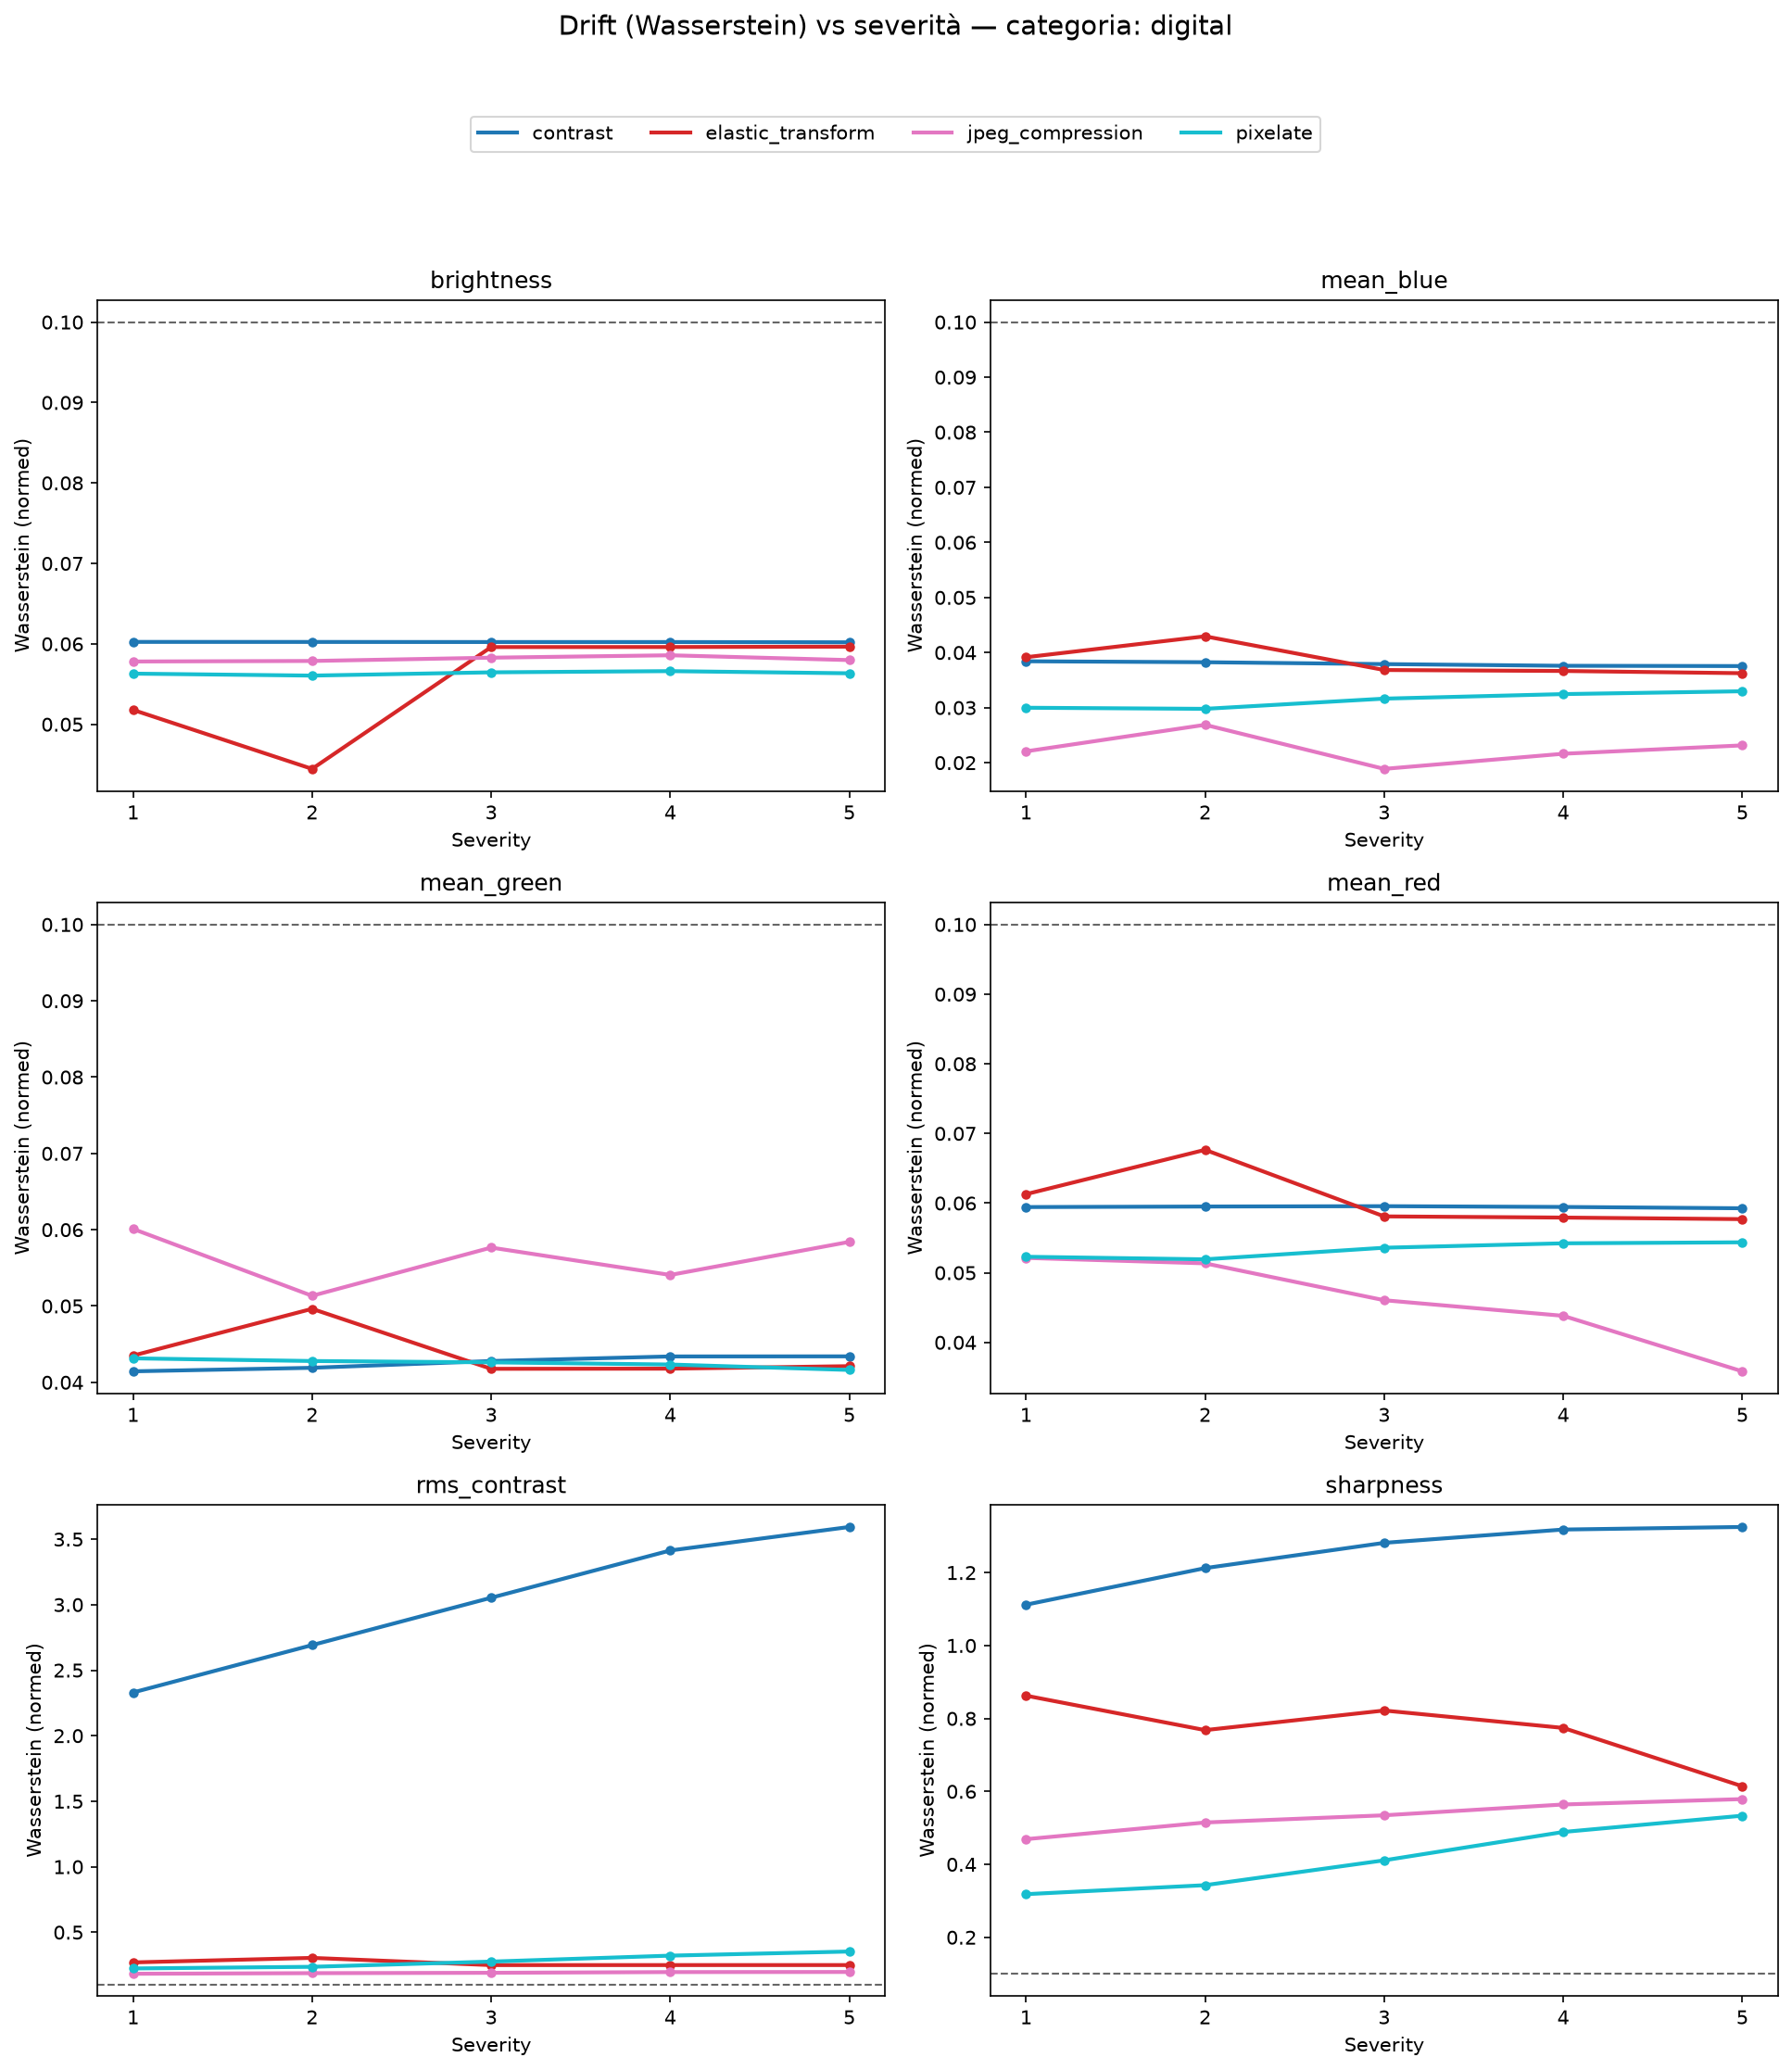
\includegraphics[width=\textwidth]{images/metrics/ImageNet-C/severity_curves/imagenet_c_severity_drift_digital.png}
	\caption{Distanza di Wesserstein tra le distribuzioni delle misure di luminanza, contrasto, nitidezza e media dei canali colore per ImageNet-C nel gruppo di corruzione digital, al variare della severità.}
	\label{fig:imagenet_c_drift_severity_digital}
\end{figure}
\begin{figure}[H]
	\centering
	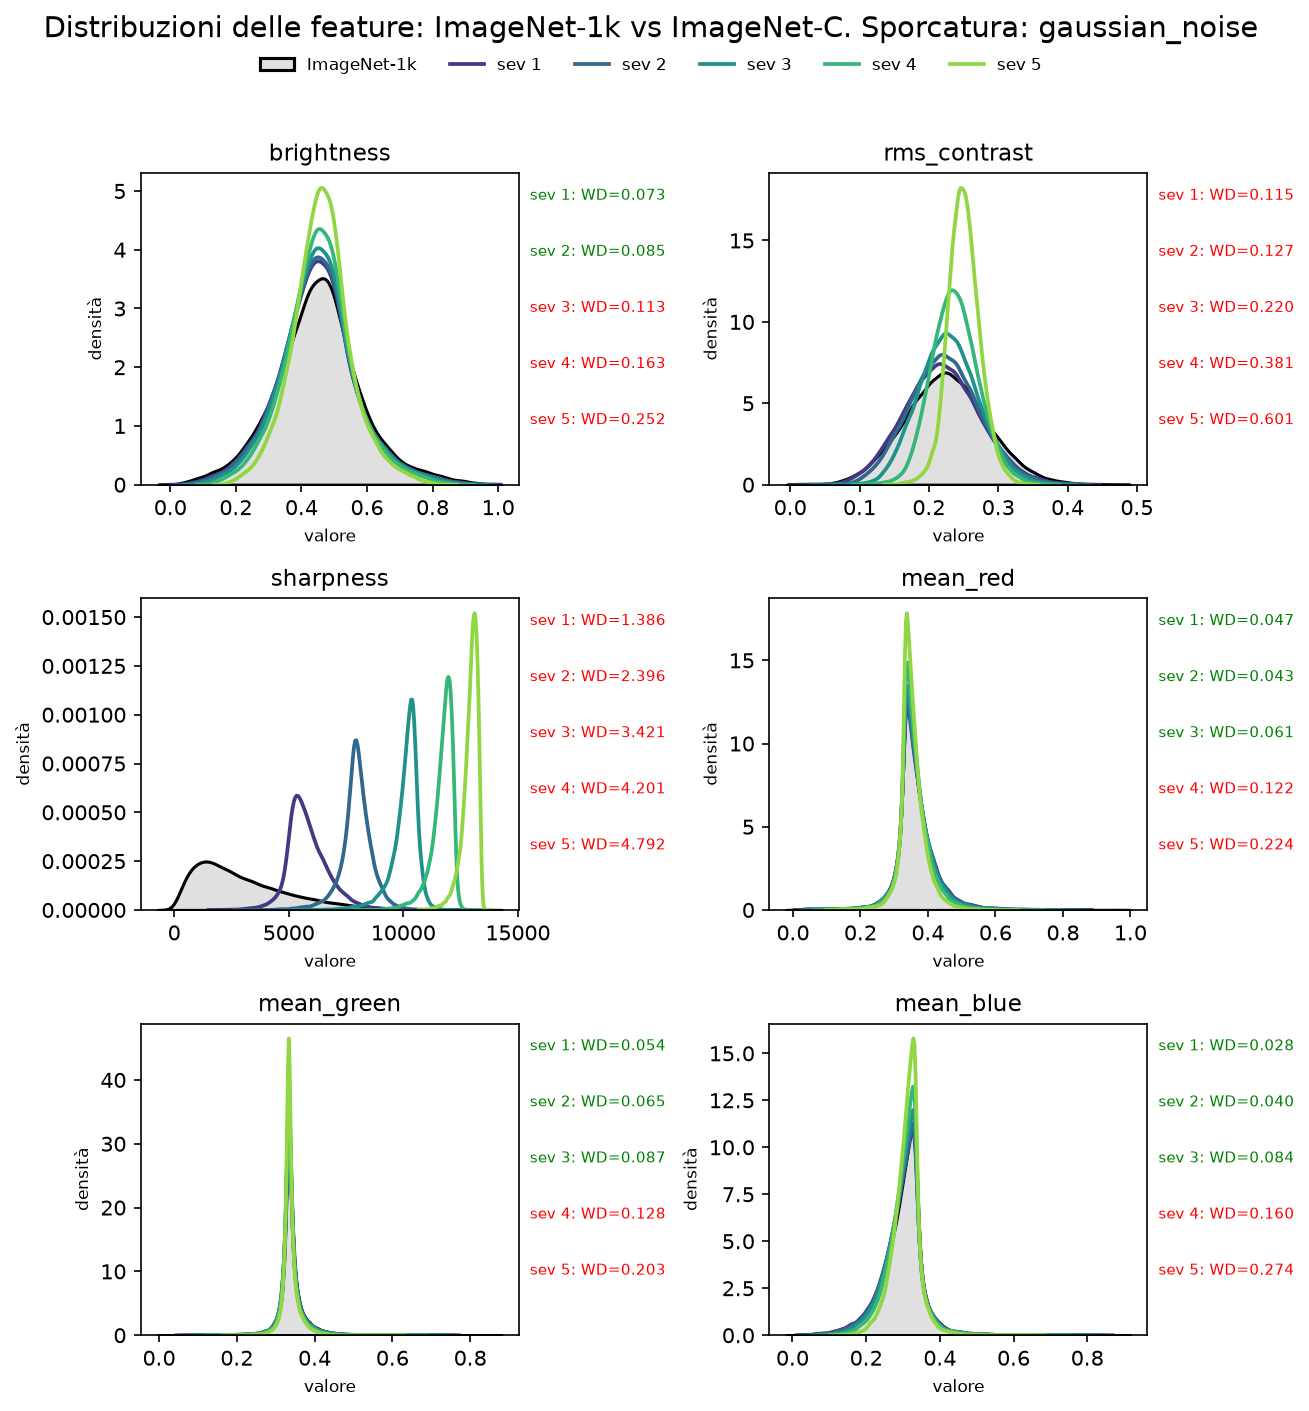
\includegraphics[width=\textwidth]{images/metrics/ImageNet-C/distributions_by_corruption/gaussian_noise.png}
	\caption{Distribuzione delle misure di luminanza, contrasto, nitidezza e media dei canali colore per ImageNet-1k e ImageNet-C con rumore gaussiano.}
	\label{fig:imagenet_c_drift_image_gaussian}
\end{figure}
\begin{figure}[H]
	\centering
	
\includegraphics[width=\textwidth]{images/metrics/ImageNet-C/distributions_by_corruption/shot_noise.png}
	\caption{Distribuzione delle misure di luminanza, contrasto, nitidezza e media dei canali colore per ImageNet-1k e ImageNet-C con rumore di shot.}
	\label{fig:imagenet_c_drift_image_shot}
\end{figure}
\begin{figure}[H]
	\centering
	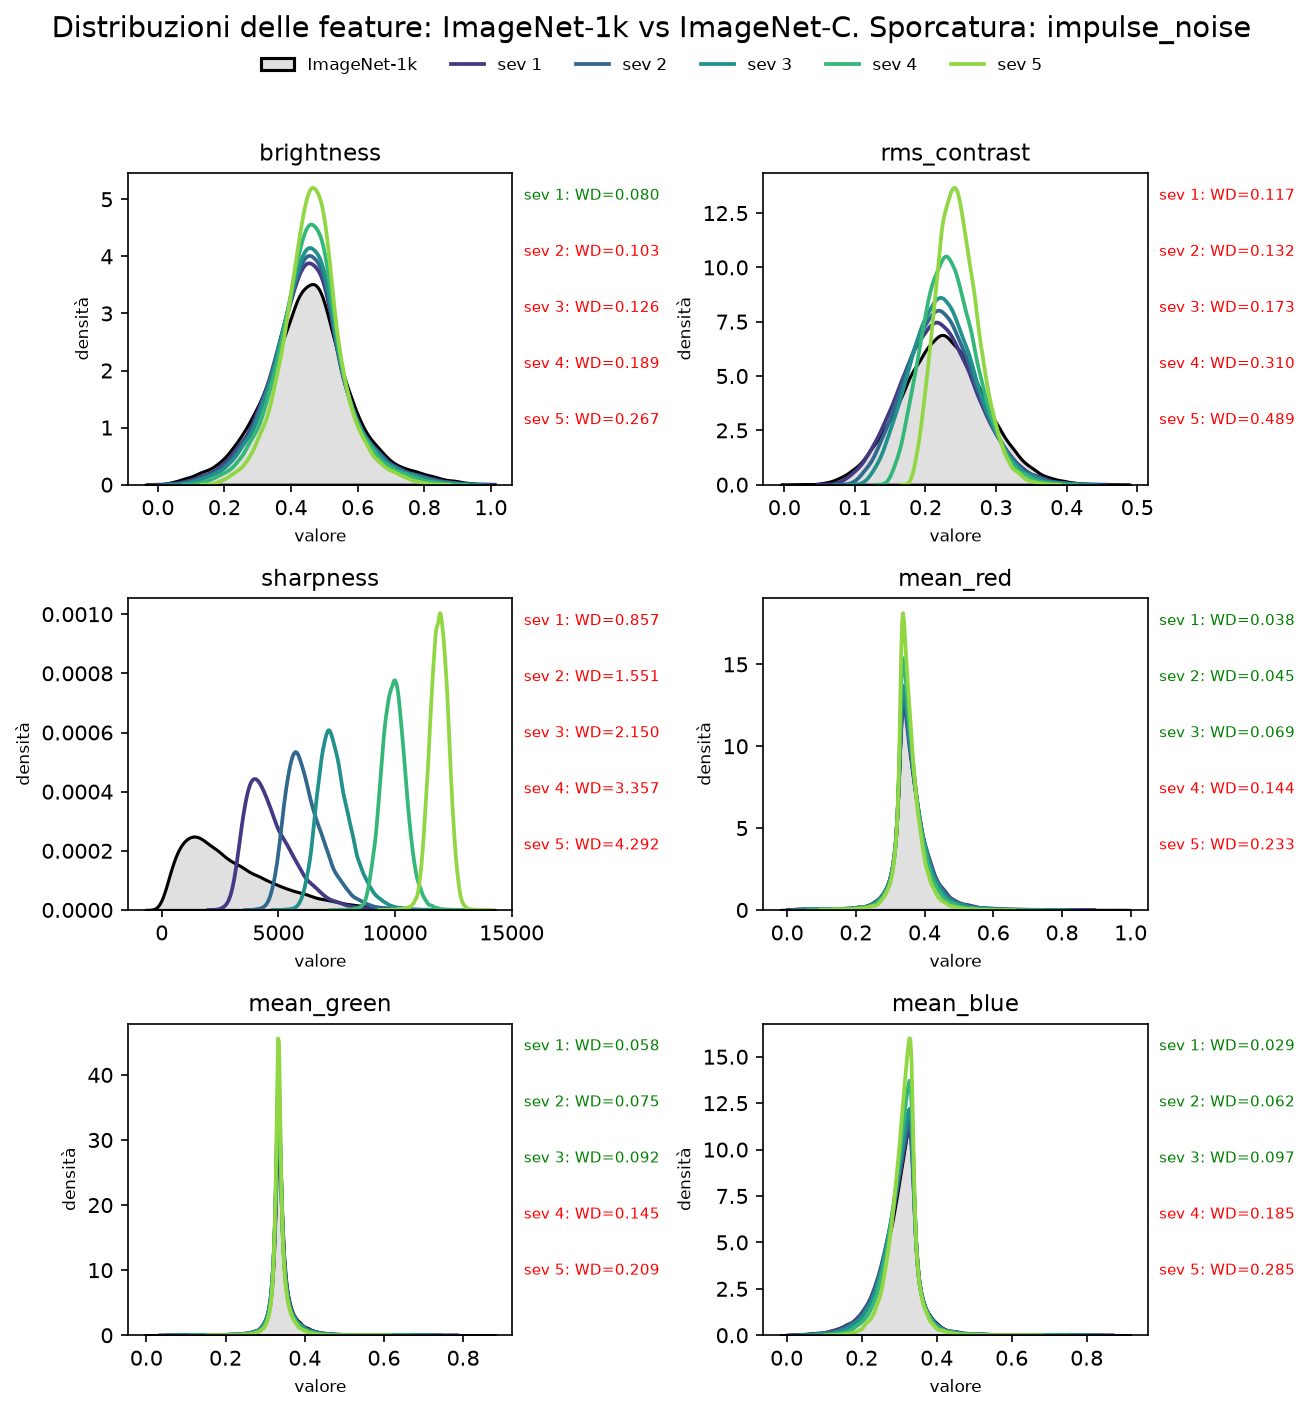
\includegraphics[width=\textwidth]{images/metrics/ImageNet-C/distributions_by_corruption/impulse_noise.png}
	\caption{Distribuzione delle misure di luminanza, contrasto, nitidezza e media dei canali colore per ImageNet-1k e ImageNet-C con rumore impulsivo.}
	\label{fig:imagenet_c_drift_image_impulse}
\end{figure}
\begin{figure}[H]
	\centering
	
\includegraphics[width=\textwidth]{images/metrics/ImageNet-C/distributions_by_corruption/defocus_blur.png}
	\caption{Distribuzione delle misure di luminanza, contrasto, nitidezza e media dei canali colore per ImageNet-1k e ImageNet-C con sfocatura da defocus.}
	\label{fig:imagenet_c_drift_image_defocus}
\end{figure}
\begin{figure}[H]
	\centering
	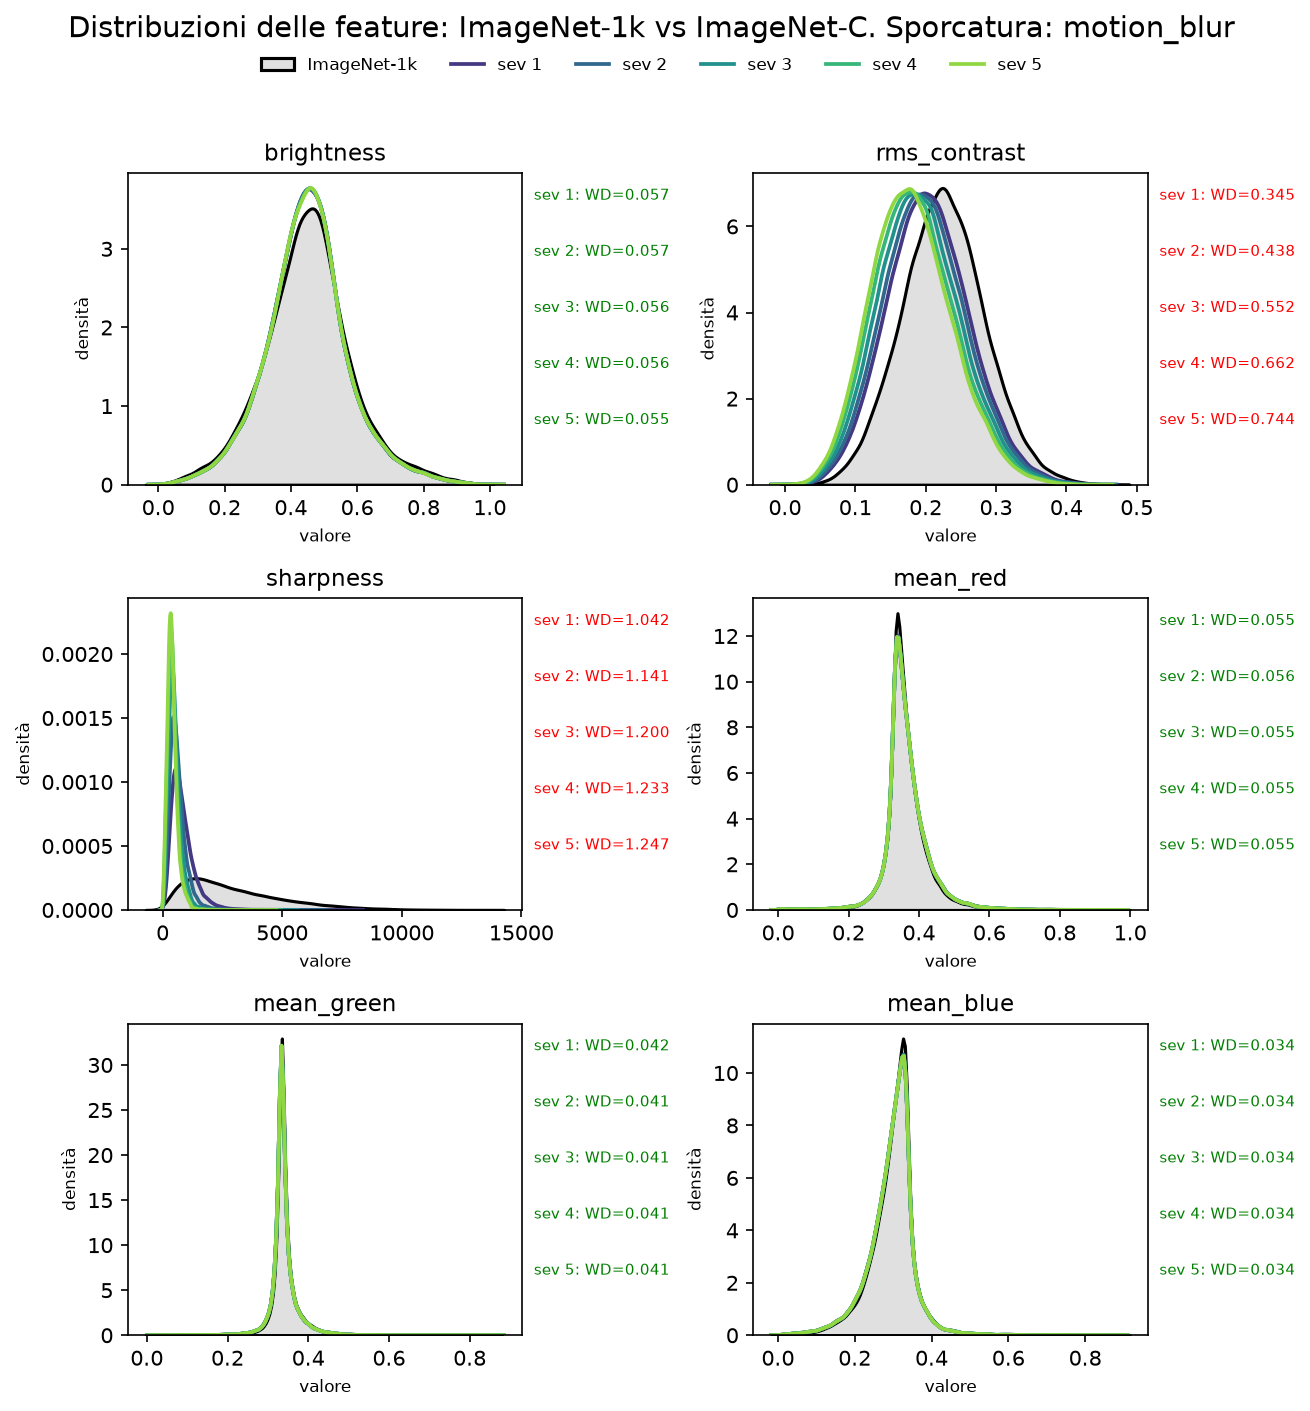
\includegraphics[width=\textwidth]{images/metrics/ImageNet-C/distributions_by_corruption/motion_blur.png}
	\caption{Distribuzione delle misure di luminanza, contrasto, nitidezza e media dei canali colore per ImageNet-1k e ImageNet-C con sfocatura da movimento.}
	\label{fig:imagenet_c_drift_image_motion}
\end{figure}
\begin{figure}[H]
	\centering
	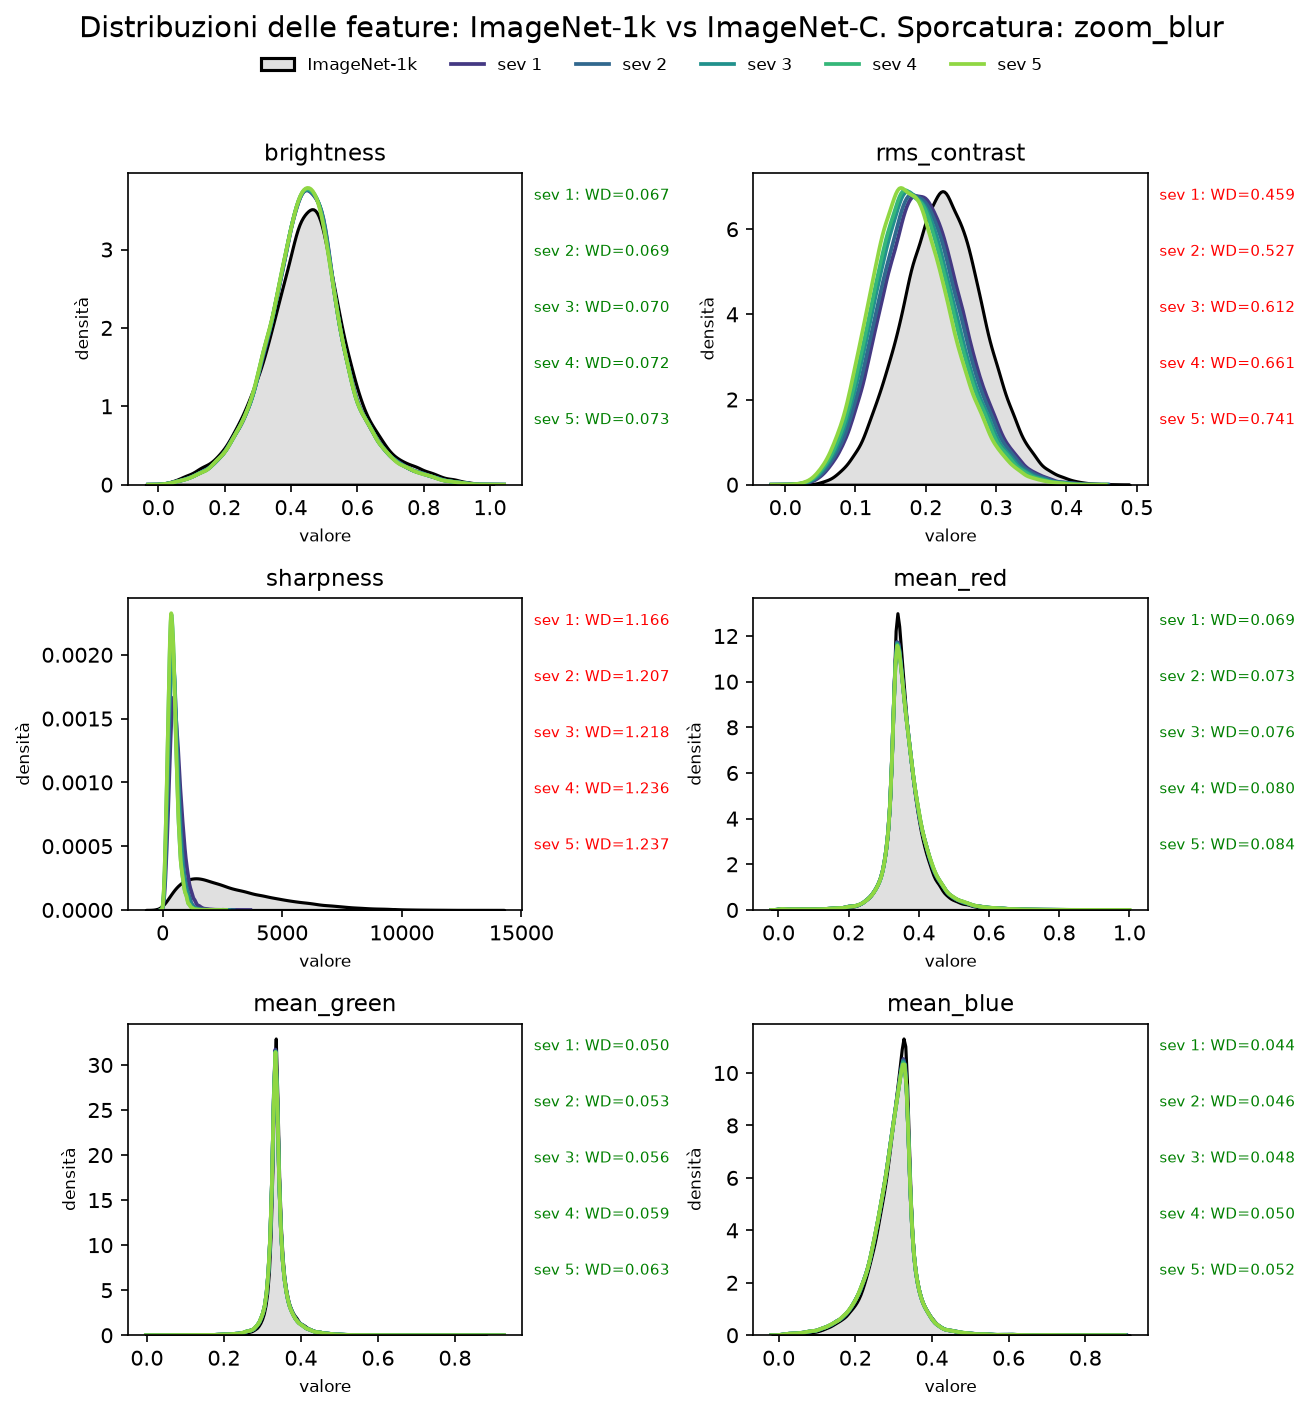
\includegraphics[width=\textwidth]{images/metrics/ImageNet-C/distributions_by_corruption/zoom_blur.png}
	\caption{Distribuzione delle misure di luminanza, contrasto, nitidezza e media dei canali colore per ImageNet-1k e ImageNet-C con sfocatura da zoom.}
	\label{fig:imagenet_c_drift_image_zoom}
\end{figure}
\begin{figure}[H]
	\centering
	
\includegraphics[width=\textwidth]{images/metrics/ImageNet-C/distributions_by_corruption/glass_blur.png}
	\caption{Distribuzione delle misure di luminanza, contrasto, nitidezza e media dei canali colore per ImageNet-1k e ImageNet-C con corruzione da vetro satinato.}
	\label{fig:imagenet_c_drift_image_glass}
\end{figure}
\begin{figure}[H]
	\centering
	
\includegraphics[width=\textwidth]{images/metrics/ImageNet-C/distributions_by_corruption/frost.png}
	\caption{Distribuzione delle misure di luminanza, contrasto, nitidezza e media dei canali colore per ImageNet-1k e ImageNet-C con corruzione da brina.}
	\label{fig:imagenet_c_drift_image_frost}
\end{figure}
\begin{figure}[H]
	\centering
	
\includegraphics[width=\textwidth]{images/metrics/ImageNet-C/distributions_by_corruption/fog.png}
	\caption{Distribuzione delle misure di luminanza, contrasto, nitidezza e media dei canali colore per ImageNet-1k e ImageNet-C con corruzione da nebbia.}
	\label{fig:imagenet_c_drift_image_fog}
\end{figure}
\begin{figure}[H]
	\centering
	
\includegraphics[width=\textwidth]{images/metrics/ImageNet-C/distributions_by_corruption/snow.png}
	\caption{Distribuzione delle misure di luminanza, contrasto, nitidezza e media dei canali colore per ImageNet-1k e ImageNet-C con corruzione da neve.}
	\label{fig:imagenet_c_drift_image_snow}
\end{figure}
\begin{figure}[H]
	\centering
	
\includegraphics[width=\textwidth]{images/metrics/ImageNet-C/distributions_by_corruption/brightness.png}
	\caption{Distribuzione delle misure di luminanza, contrasto, nitidezza e media dei canali colore per ImageNet-1k e ImageNet-C con corruzione da luminosità.}
	\label{fig:imagenet_c_drift_image_brightness}
\end{figure}
\begin{figure}[H]
	\centering
	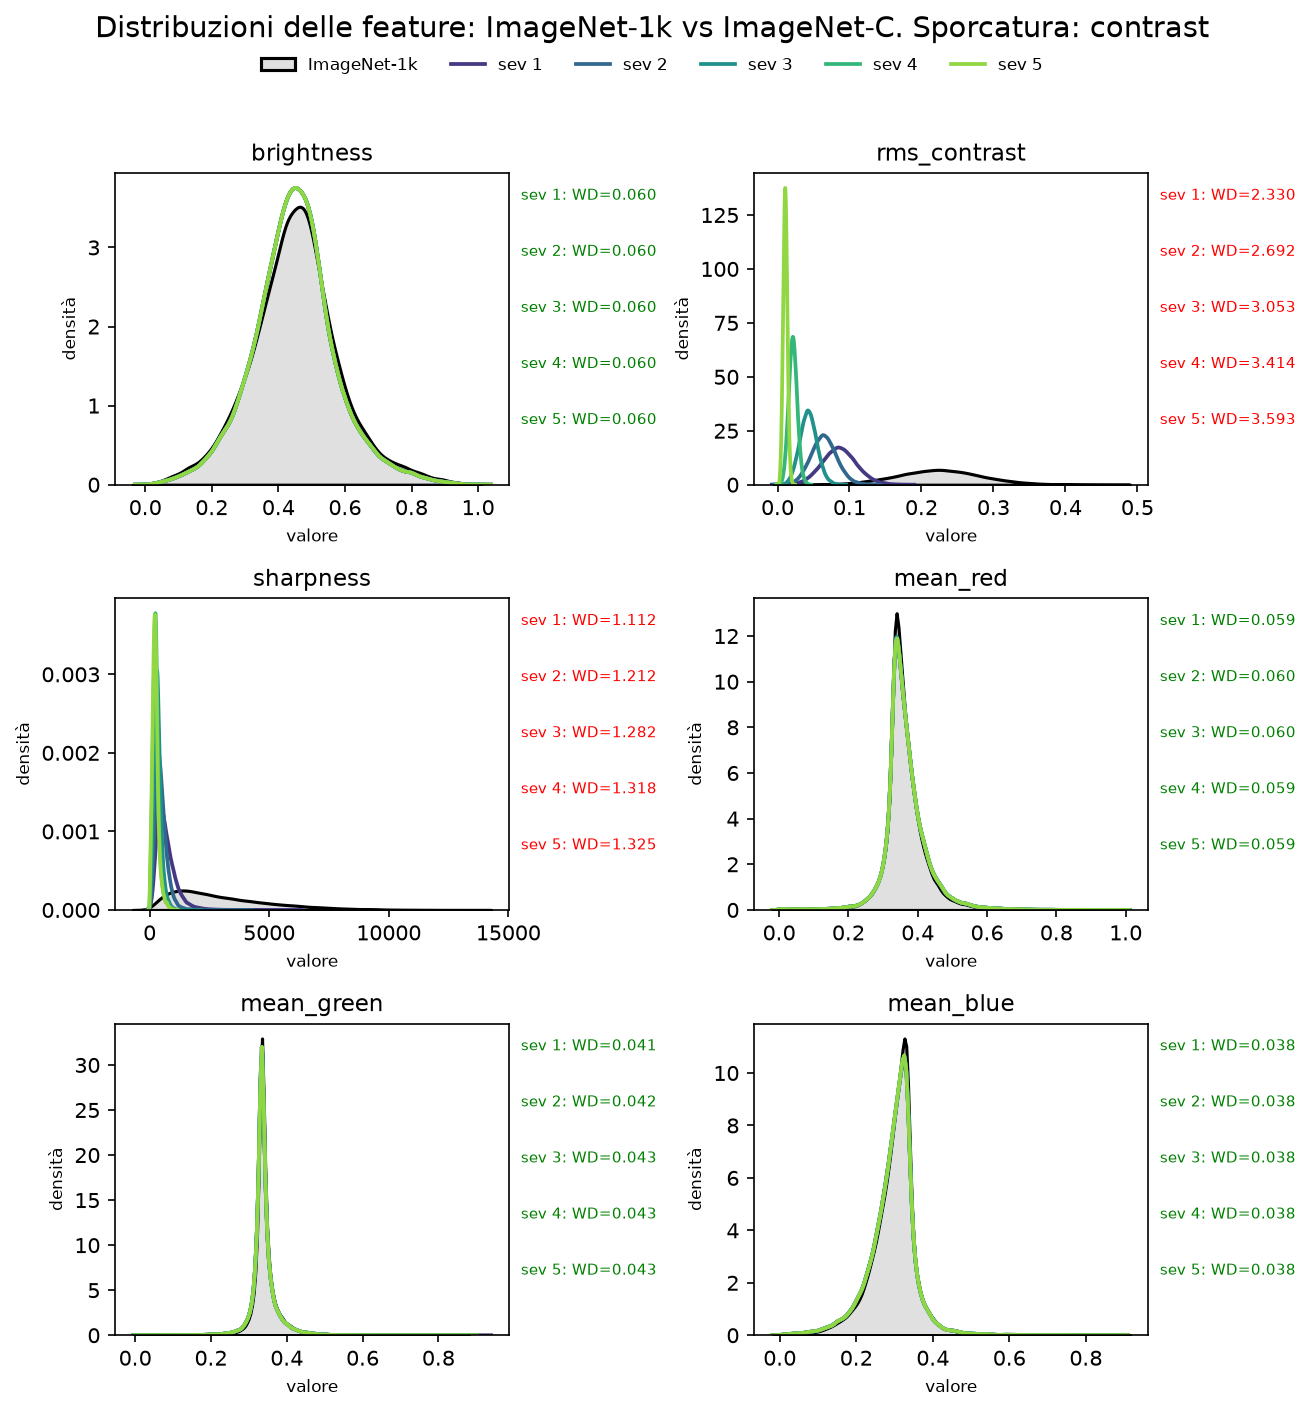
\includegraphics[width=\textwidth]{images/metrics/ImageNet-C/distributions_by_corruption/contrast.png}
	\caption{Distribuzione delle misure di luminanza, contrasto, nitidezza e media dei canali colore per ImageNet-1k e ImageNet-C con corruzione da contrasto.}
	\label{fig:imagenet_c_drift_image_contrast}
\end{figure}
\begin{figure}[H]
	\centering
	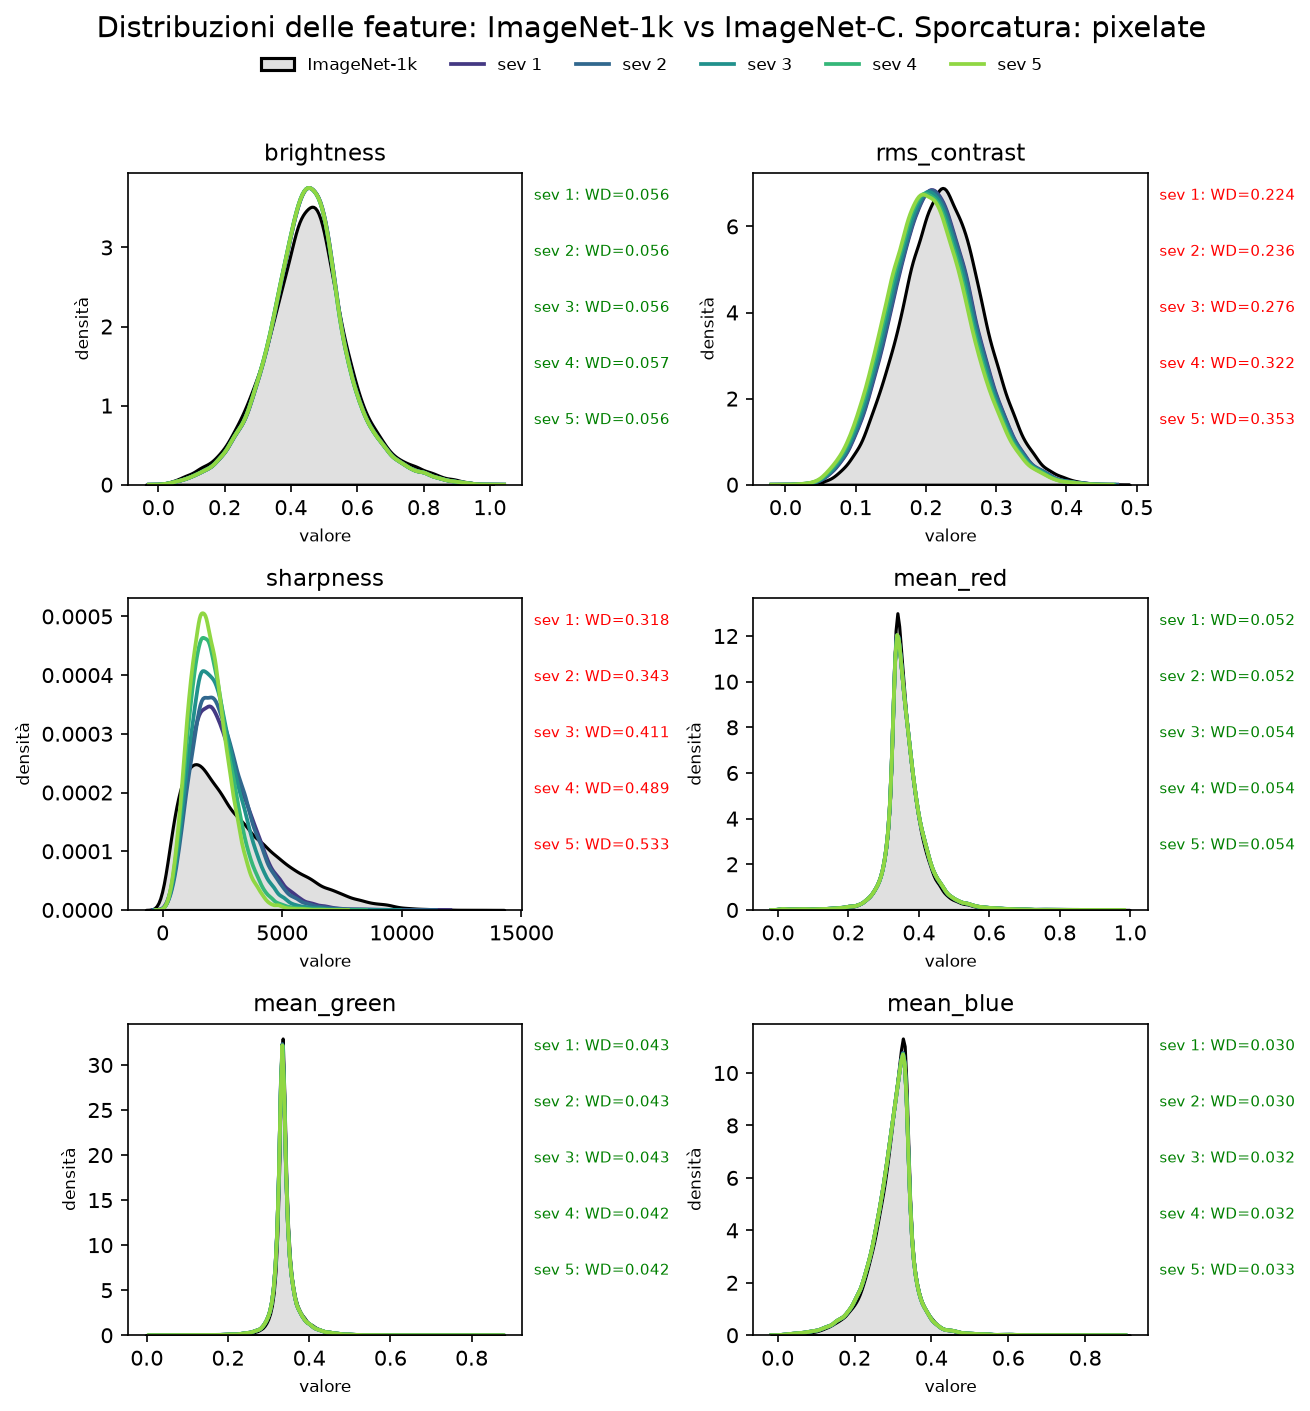
\includegraphics[width=\textwidth]{images/metrics/ImageNet-C/distributions_by_corruption/pixelate.png}
	\caption{Distribuzione delle misure di luminanza, contrasto, nitidezza e media dei canali colore per ImageNet-1k e ImageNet-C con corruzione da pixelizzazione.}
	\label{fig:imagenet_c_drift_image_pixelate}
\end{figure}
\begin{figure}[H]
	\centering
	
\includegraphics[width=\textwidth]{images/metrics/ImageNet-C/distributions_by_corruption/jpeg_compression.png}
	\caption{Distribuzione delle misure di luminanza, contrasto, nitidezza e media dei canali colore per ImageNet-1k e ImageNet-C con corruzione da compressione JPEG.}
	\label{fig:imagenet_c_drift_image_jpeg}
\end{figure}
\begin{figure}[H]
	\centering
	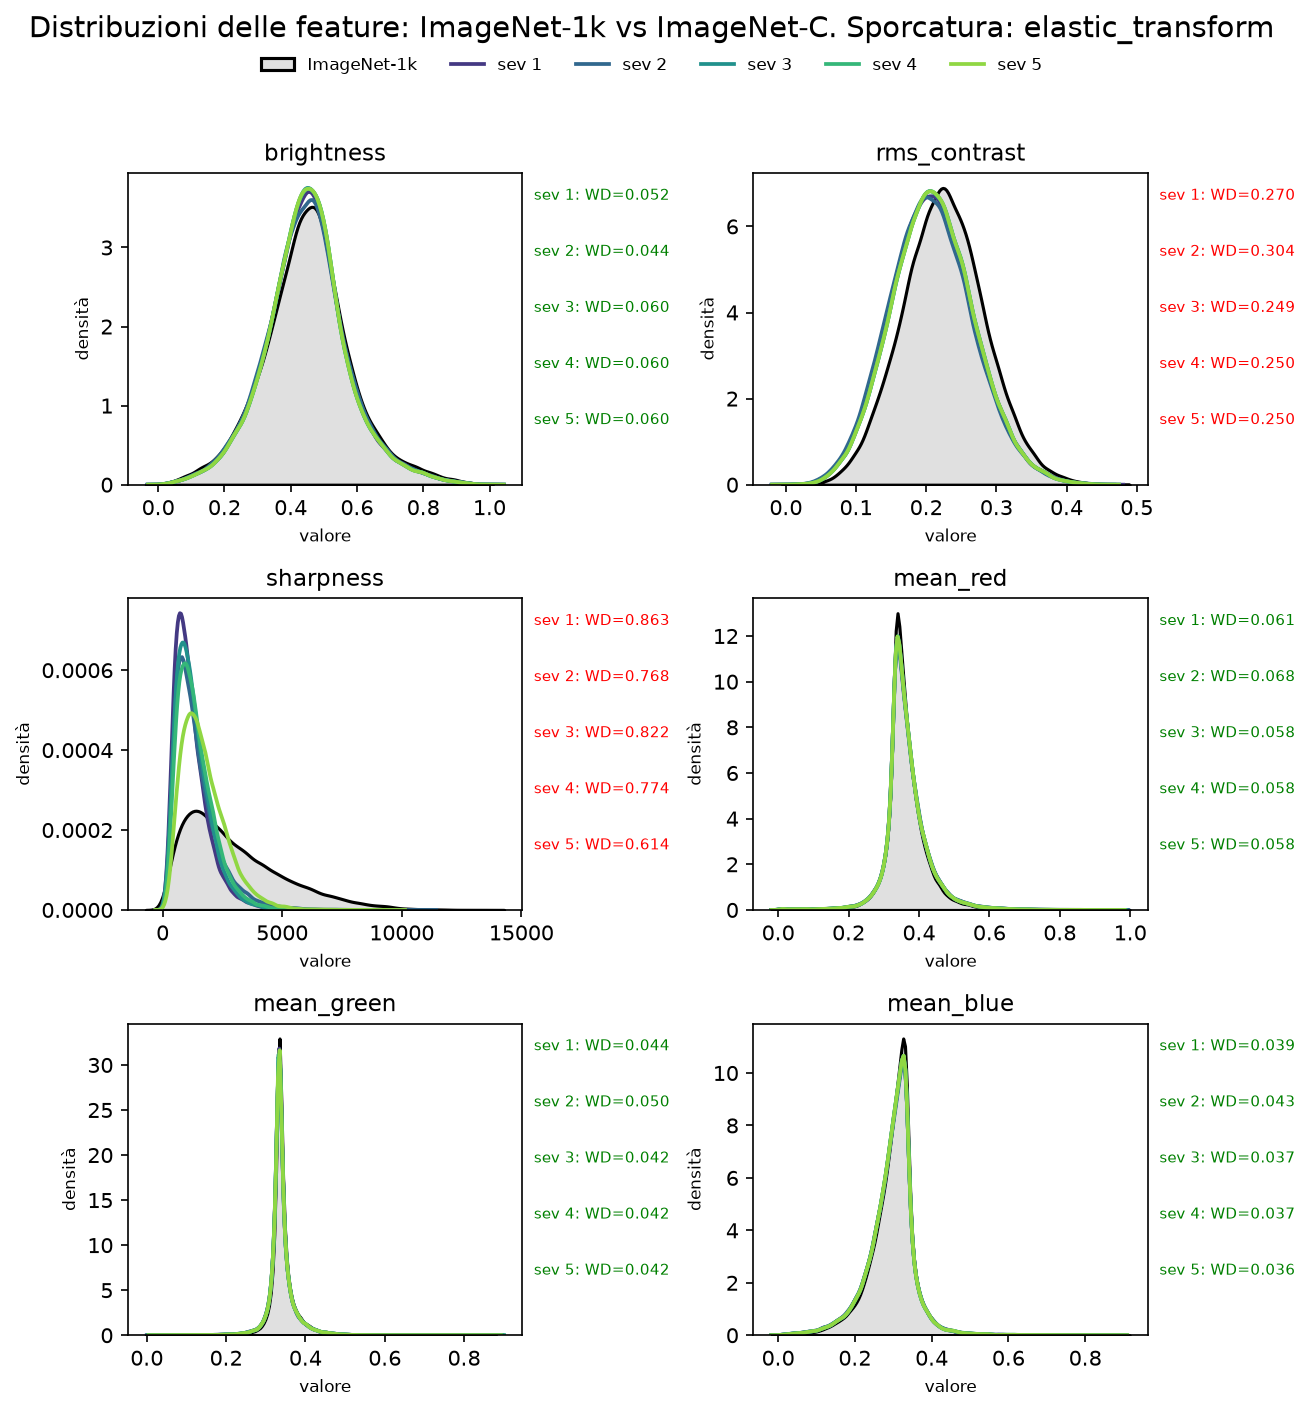
\includegraphics[width=\textwidth]{images/metrics/ImageNet-C/distributions_by_corruption/elastic_transform.png}
	\caption{Distribuzione delle misure di luminanza, contrasto, nitidezza e media dei canali colore per ImageNet-1k e ImageNet-C con corruzione da trasformazione elastica.}
	\label{fig:imagenet_c_drift_image_elastic}
\end{figure}
\section{Analisi delle metriche di drift sulle feature del modello}
In questa sezione vengono analizzate le metriche di drift calcolate sulle feature del modello ResNet-50, estratte dal layer \texttt{avgpool}. Come già accennato nella sezione 4, la rilevazione delle feature viene effettuata tramite test MMD.I test sono stati effettuati con un valore di soglia uguale a $0.05$, quindi viene rilevato un drift quando il p-value $p < 0.05$
\subsection{ImageNet-1k vs ImageNet-R}
Il test MMD ImageNet-R è stato effettuato rispetto alle feature ottenute dalla classificazione di ImageNet-1k sottocampionato alle duecento classi in comune con ImageNet-R.
\begin{table}[H]
  \centering
  \begin{tabular}{llll}
    \toprule
    dataset & is\_drift & p\_val & distance \\
    \midrule
    ImageNetR & True & 0.0000 & 0.0805 \\ 
    \bottomrule
  \end{tabular}
	\caption{Risultati del test di MMD tra le feature estratte dal layer \texttt{avgpool} del modello ResNet-50 per ImageNet-1k e ImageNet-R.}
	\label{tab:mmd_drift_report}
\end{table}
Come si può notare dal risultato riportato in tabella \ref{tab:mmd_drift_report}, il p-value del test è zero, quindi al di sotto della soglia di rilevazione. La rilevazione del drift è quindi coerente con il drift rilevato per le feature visive, come si può
vedere in figura \ref{fig:imagenet_r_drift_image}.
\subsection{ImageNet-1k vs ImageNet-C}
Per poter fare l'analisi di MMD delle feature, è stato necessario effettuare un campionamento a 10.000 esempi, in quanto utilizzare l'intero dataset avrebbe richiesto una quantità di memoria della GPU a noi non disponibile. Il campionamento è casuale, mantenendo un numero equo di esempi per ogni classe. 

Analizziamo ora le metriche di drift rilevate nelle feature utilizzate dal modello durante la classificazione e confrontiamo il risultato con il drift rilevato nelle feature visive.
\subsubsection{Blur}
\begin{table}[H]
  \centering
  \begin{tabular}{lllll}
    \toprule
    corruption & severity & is\_drift & p\_val & distance \\
    \midrule
    defocus\_blur & 1 & True & 0.0000 & 0.0002 \\ 
    defocus\_blur & 2 & True & 0.0000 & 0.0003 \\ 
    defocus\_blur & 3 & True & 0.0000 & 0.0005 \\ 
    defocus\_blur & 4 & True & 0.0000 & 0.0009 \\ 
    defocus\_blur & 5 & True & 0.0000 & 0.0022 \\ 
    glass\_blur & 1 & True & 0.0000 & 0.0002 \\ 
    glass\_blur & 2 & True & 0.0000 & 0.0031 \\ 
    glass\_blur & 3 & True & 0.0000 & 0.0176 \\ 
    glass\_blur & 4 & True & 0.0000 & 0.0321 \\ 
    glass\_blur & 5 & True & 0.0000 & 0.0238 \\ 
    motion\_blur & 1 & False & 0.2000 & 0.0000 \\ 
    motion\_blur & 2 & False & 0.1500 & 0.0001 \\ 
    motion\_blur & 3 & True & 0.0000 & 0.0013 \\ 
    motion\_blur & 4 & True & 0.0000 & 0.0099 \\ 
    motion\_blur & 5 & True & 0.0000 & 0.0229 \\ 
    zoom\_blur & 1 & True & 0.0000 & 0.0006 \\ 
    zoom\_blur & 2 & True & 0.0000 & 0.0021 \\ 
    zoom\_blur & 3 & True & 0.0000 & 0.0017 \\ 
    zoom\_blur & 4 & True & 0.0000 & 0.0027 \\ 
    zoom\_blur & 5 & True & 0.0000 & 0.0013 \\ 
    \bottomrule
  \end{tabular}
\caption{Risultati del test di MMD tra le feature estratte dal layer \texttt{avgpool} del modello ResNet-50 per ImageNet-1k e ImageNet-C, corruzione di tipo blur.}
\label{tab:mmd_drift_report_imagenet_c_blur}
\end{table}
Per quanto riguarda la classe di sporcature blur, abbiamo ottenuto i risultati presentati in tabella \ref{tab:mmd_drift_report_imagenet_c_blur}. Possiamo effettuare le seguenti osservazioni:
\begin{itemize}
  \item \textbf{defocus\_blur}: Il drift viene rilevato ad ogni livello di severity; il ché è coerente con il drift rilevato nelle feature visive, come presentato in figura \ref{fig:imagenet_c_drift_image_defocus}. Infatti, in questo tipo di sporcatura sharpness e rms\_contrast presentano un drift a tutti i livelli di severity.
  \item \textbf{glass\_blur}: Come si può notare in figura \ref{fig:imagenet_c_drift_image_glass}, le feature sharpness e rms\_contrast presentano un drift a tutti i livelli di severity. Valgono quindi le stesse considerazioni effettuate per defocus\_blur.
  \item \textbf{motion\_blur}: Nonostante venga rilevato, come nelle due sporcature precedenti e riportato in figura \ref{fig:imagenet_c_drift_image_motion}, un drift nelle feature sharpness e rms\_contrast in tutti di livelli di severità, con distanze di Wesserstein simili a quelle rilevate per defocus\_blur e glass\_blur, le feature estratte dal modello per i primi due livelli non presentano drift rispetto alle feature estratte da ImageNet-1k. Infatti, le feature che il modello estrae e utilizza per la classificazione sono fondamentalmente diverse rispetto a quelle estraibili direttamente dalle immagini, quindi è possibile che, nonostante la sporcatura, le feature estratte per i primi due livelli di severità non presentino drift rispetto a quelle estratte per imagenet-1k.
  \item \textbf{zoom\_blur}: Valgono le stesse considerazioni effettuate per defocus\_blur e glass\_blur. Ciò si può notare osservando la figura \ref{fig:imagenet_c_drift_image_zoom}.
\end{itemize}
\subsubsection{Digital}

\begin{table}[H]
  \centering
  \begin{tabular}{lllll}
    \toprule
    corruption & severity & is\_drift & p\_val & distance \\
    \midrule
    contrast & 1 & False & 0.2500 & 0.0000 \\ 
    contrast & 2 & False & 0.1500 & 0.0001 \\ 
    contrast & 3 & False & 0.1500 & 0.0001 \\ 
    contrast & 4 & True & 0.0000 & 0.0005 \\ 
    contrast & 5 & True & 0.0000 & 0.0029 \\ 
    elastic\_transform & 1 & False & 0.2500 & 0.0001 \\ 
    elastic\_transform & 2 & True & 0.0000 & 0.0011 \\ 
    elastic\_transform & 3 & True & 0.0000 & 0.0017 \\ 
    elastic\_transform & 4 & True & 0.0000 & 0.0083 \\ 
    elastic\_transform & 5 & True & 0.0000 & 0.0740 \\ 
    jpeg\_compression & 1 & False & 0.0500 & 0.0001 \\ 
    jpeg\_compression & 2 & False & 0.1500 & 0.0001 \\ 
    jpeg\_compression & 3 & False & 0.1000 & 0.0002 \\ 
    jpeg\_compression & 4 & False & 0.0500 & 0.0002 \\ 
    jpeg\_compression & 5 & False & 0.0500 & 0.0002 \\ 
    pixelate & 1 & False & 0.2000 & 0.0001 \\ 
    pixelate & 2 & True & 0.0000 & 0.0002 \\ 
    pixelate & 3 & True & 0.0000 & 0.0005 \\ 
    pixelate & 4 & True & 0.0000 & 0.0020 \\ 
    pixelate & 5 & True & 0.0000 & 0.0126 \\ 
    \bottomrule
  \end{tabular}
\caption{Risultati del test di MMD tra le feature estratte dal layer \texttt{avgpool} del modello ResNet-50 per ImageNet-1k e ImageNet-C, corruzione di tipo digital.}
\label{tab:mmd_drift_report_imagenet_c_digital}
\end{table}
Per quanto riguarda la classe di sporcature digital, abbiamo ottenuto i risultati presentati in tabella \ref{tab:mmd_drift_report_imagenet_c_digital}. Possiamo effettuare le seguenti osservazioni:
\begin{itemize}
  \item \textbf{contrast}: A differenza di quanto rilevato per le feature visive rms\_contrast e sharpness, come si può vedere in figura \ref{fig:imagenet_c_drift_image_contrast}, il test MMD non rileva una presenza di drift nelle feature ai primi tre livello di severità. Valgono quindi le stesse considerazioni effettuate per motion\_blur.
  \item \textbf{eleastic\_transform}: Come rilevato per contrast, vi è una discrepanza fra il drift rilevato nelle feature visive, riportato in figura \ref{fig:imagenet_c_drift_image_elastic}, e il drift rilevato nelle feature estratte dal modello. In particolare, esse non risultano soggette a drift per il primo livello di severity.
  \item \textbf{jpeg\_compression}: Per questo tipo di sporcatura, le feature estratte dal modello non risultano soggette a drift per nessun livello di severity, nonostante le feature visive rms\_contrast e sharpness risultino soggette a drift, seppur con distanza di Wesserstein più bassa rispetto ad altri tipi di sporcatura. Ciò è riportato in figura \ref{fig:imagenet_c_drift_image_jpeg}. Questo è dato probabilmente dal fatto che le feature estratte per questo tipo di sporcature presentino un drift minimo o nullo rispetto alle feature di riferimento.
  \item \textbf{pixelate}: A differenza di quanto rilevato per le feature visive rms\_contrast e sharpness, riportato in figura \ref{fig:imagenet_c_drift_image_pixelate}, le feature estratte dal modello presentano drift solo nel primo livello di severity. Valgono quindi le considerazioni fatte in precedenza.
\end{itemize}
\subsubsection{Noise}
\begin{table}[H]
  \centering
  \begin{tabular}{lllll}
    \toprule
    corruption & severity & is\_drift & p\_val & distance \\
    \midrule
    gaussian\_noise & 1 & False & 0.5000 & 0.0000 \\ 
    gaussian\_noise & 2 & True & 0.0000 & 0.0005 \\ 
    gaussian\_noise & 3 & True & 0.0000 & 0.0025 \\ 
    gaussian\_noise & 4 & True & 0.0000 & 0.0110 \\ 
    gaussian\_noise & 5 & True & 0.0000 & 0.0682 \\ 
    impulse\_noise & 1 & True & 0.0000 & 0.0004 \\ 
    impulse\_noise & 2 & True & 0.0000 & 0.0014 \\ 
    impulse\_noise & 3 & True & 0.0000 & 0.0040 \\ 
    impulse\_noise & 4 & True & 0.0000 & 0.0215 \\ 
    impulse\_noise & 5 & True & 0.0000 & 0.0840 \\ 
    shot\_noise & 1 & False & 0.2000 & 0.0000 \\ 
    shot\_noise & 2 & True & 0.0000 & 0.0005 \\ 
    shot\_noise & 3 & True & 0.0000 & 0.0028 \\ 
    shot\_noise & 4 & True & 0.0000 & 0.0155 \\ 
    shot\_noise & 5 & True & 0.0000 & 0.0433 \\ 
    \bottomrule
  \end{tabular}
\caption{Risultati del test di MMD tra le feature estratte dal layer \texttt{avgpool} del modello ResNet-50 per ImageNet-1k e ImageNet-C, corruzione di tipo noise.}
\label{tab:mmd_drift_report_imagenet_c_noise}
\end{table}
Per quanto riguarda la classe di sporcature noise, abbiamo ottenuto i risultati presentati in tabella \ref{tab:mmd_drift_report_imagenet_c_noise}. Possiamo effettuare le seguenti osservazioni:
\begin{itemize}
  \item \textbf{gaussian\_noise}: Per questo tipo di sporcatura, le feature visive rms\_contrast, sharpness presentano sempre un drift, le medie dei canali colore presentano un drift dal quarto livello di severità in poi e brightness presenta un drift dal terzo livello di severità in poi. Questi risultati sono riportati in figura \ref{fig:imagenet_c_drift_image_gaussian}. A differenza di quanto rilevato nelle feature visive, le feature estratte dal modello presentano un drift solamente dal secondo livello di severità. Come quindi già detto in precedenza, le feature estratte dal modello per il primo livello di severità sono uguali a quelle estratte per ImageNet-1k, infatti la distanza MMD rilevata è $0$.
  \item \textbf{impulse\_noise}: Per questo tipo di sporcatura, le feature visive rms\_contrast e sharpness presentano sempre un drift, le medie dei canali colore presentano un drift dal quarto livello di severità e brightness dal secondo livello di severità. Ciò è riportato nella figura \ref{fig:imagenet_c_drift_image_impulse}. Come rilevato in precedenza, vi è quindi una discrepanza tra il drift rilevato nelle feature visive e quello rilevato nelle feature estratte dal modello: infatti, quest'ultime presentano sempre un drift rispetto alle feature di riferimento.
  \item \textbf{shot\_noise}: Per questo tipo di sporcatura, le feature visive rms\_contrast e sharpness presentano sempre un drift, brightness presenta un drift dal terzo livello di severità in poi. A differenza degli altri tipi di sporcatura in questa classe, l'unica media del canale colore che presenta un drift è quella del canale blu all'ultimo livello di severity.
  Anche in questo caso, il drift rilevato nelle feature estratte dal modello diverge rispetto a quanto rilevato nelle feature visive: infatti, viene rilevato un drift solamente dal secondo livello di severità. 
\end{itemize}
\subsubsection{Weather}
\begin{table}[H]
  \centering
  \begin{tabular}{lllll}
    \toprule
    corruption & severity & is\_drift & p\_val & distance \\
    \midrule
    brightness & 1 & False & 0.3500 & 0.0000 \\ 
    brightness & 2 & False & 0.1000 & 0.0001 \\ 
    brightness & 3 & False & 0.1000 & 0.0000 \\ 
    brightness & 4 & False & 0.2500 & 0.0001 \\ 
    brightness & 5 & True & 0.0000 & 0.0003 \\ 
    fog & 1 & False & 0.3500 & 0.0000 \\ 
    fog & 2 & False & 0.1500 & 0.0001 \\ 
    fog & 3 & False & 0.2500 & 0.0001 \\ 
    fog & 4 & False & 0.1000 & 0.0002 \\ 
    fog & 5 & True & 0.0000 & 0.0021 \\ 
    frost & 1 & False & 0.1500 & 0.0000 \\ 
    frost & 2 & True & 0.0000 & 0.0004 \\ 
    frost & 3 & True & 0.0000 & 0.0016 \\ 
    frost & 4 & True & 0.0000 & 0.0020 \\ 
    frost & 5 & True & 0.0000 & 0.0043 \\ 
    snow & 1 & True & 0.0000 & 0.0003 \\ 
    snow & 2 & True & 0.0000 & 0.0010 \\ 
    snow & 3 & True & 0.0000 & 0.0032 \\ 
    snow & 4 & True & 0.0000 & 0.0050 \\ 
    snow & 5 & True & 0.0000 & 0.0133 \\ 
    \bottomrule
  \end{tabular}
\caption{Risultati del test di MMD tra le feature estratte dal layer \texttt{avgpool} del modello ResNet-50 per ImageNet-1k e ImageNet-C, corruzione di tipo weather.}
\label{tab:mmd_drift_report_imagenet_c_weather}
\end{table}
Per quanto riguarda la classe di sporcature weather, abbiamo ottenuto i risultati presentati in tabella \ref{tab:mmd_drift_report_imagenet_c_weather}. Possiamo effettuare le seguenti osservazioni:
\begin{itemize}
  \item \textbf{brightness}: Per questo tipo di sporcatura, si presenta un drift in tutte le feature visive e a tutti i livelli di severity tranne per le medie dei canali colore, le quali non presentano alcun tipo di drift. Ciò è riportato in figura \ref{fig:imagenet_c_drift_image_brightness}. Come si può osservare dalla tabella \ref{tab:mmd_drift_report_imagenet_c_weather}, le feature estratte dal modello presentano un drift rispetto a quelle estratte da ImageNet-1k solamente al quinto livello di severity. Valgono quindi le considerazioni effettuate in precedenza sulle feature estratte dal modello.
  \item \textbf{fog}: Per questo tipo di sporcatura, tutte le feature visive presentano un drift a tutti i livelli di severità. La figura \ref{fig:imagenet_c_drift_image_fog} presenta il drift misurato su queste feature. Ciò non si riflette nelle feature estratte dal modello, nelle quali viene rilevato un drift dal test MMD solamente al quinti livello di severità.
  \item \textbf{frost}: Per questo tipo di sporcatura, tutte le feature visive presentano un drift a tutti i livelli di severità. La figura \ref{fig:imagenet_c_drift_image_frost} presenta il drift misurato su queste feature. Ciò si riflette solamente parzialmente sulle feature estratte dal modello: infatti, viene rilevato un drift in esse solamente dal secondo livello di severità.
  \item \textbf{snow}: Per questo tipo di sporcatura, tutte le feature visive presentano un drift a tutti i livelli di severità tranne rms\_contrast, la quale presenta un drift solamente a partire dal secondo livello di severità. La figura \ref{fig:imagenet_c_drift_image_snow} presenta il drift misurato su queste feature. Ciò si riflette quindi solamente parzialmente sulle feature estratte dal modello: infatti, viene rilevato un drift in esse a tutti i livelli di severità.
\end{itemize}
\subsubsection{Analisi del confronto tra tipi di feature}
Confrontando i risultati ottenuti per la rilevazione del drift sulle feature visive e sulle feature estratte dal modello, si può evincere che non vi è una correlazione diretta tra la presenza di drift nelle due. Ciò può essere dato dal fatto che la rete convolutiva computa e utilizza feature map le quali non sono direttamente confrontabili con le feature visive direttamente estratte dall'immagine, nonostante esse possano venir utilizzate per calcolare le feature map. Il drift delle feature del modello non sembra quindi essere influenzato dal drift nelle feature visive.
\section{Analisi delle performance del modello}
In questa sezione vengono analizzate le performance del modello ResNet-50 su ImageNet-R e ImageNet-C. Per ImageNet-R, confronteremo le metriche ottenute dalla classificazione delle immagini del dataset con le metriche ottenute dalla classificazione delle immagini di ImageNet-1k. Per ImageNet-C, invece, analizzeremo l'accuracy del modello al variare della severità della corruzione, calcolando la degradazione delle performance rispetto alla severity, calcolando la robustezza del modello e misurando quanto linearmente la severità della corruzione influisca sulla degradazione delle performance del modello.
\subsection{ImageNet-1k vs ImageNet-R}

\subsection{ImageNet-1k vs ImageNet-C}
\printbibliography
\end{document}